%% Submission manuscript for Operations Research Forum (Springer Nature).
%% Uses the standard article class; the journal recommends but does not require
%% its own template. Every \todo placeholder must be resolved before submission.
\documentclass[11pt,a4paper]{article}

\usepackage[margin=1in]{geometry}
\usepackage{amsmath,amssymb,booktabs,array,graphicx,microtype}
\usepackage{float}
\usepackage{xcolor}
\usepackage{caption}
\captionsetup[figure]{name={Fig.},labelfont=bf,labelsep=space}
\captionsetup[table]{labelfont=bf,labelsep=space}
\usepackage[numbers,sort&compress]{natbib}
\usepackage{hyperref}
\hypersetup{colorlinks=true,linkcolor={blue!55!black},citecolor={blue!55!black},
  urlcolor={blue!55!black},bookmarksnumbered=true,
  pdftitle={Reliability-Screened Routing Under Predictable and Stochastic Travel Variation},
  pdfauthor={Suhan Ali}}

\newcommand{\todo}[1]{\textcolor{red}{[#1]}}
%% Hook expected by Springer Nature bibliography styles; empty outside their class.
\providecommand{\bibcommenthead}{}

\newcommand{\ProcConsRange}{8.3--21.4}
\newcommand{\ConservativeSelected}{25}
\newcommand{\ConservativeRetained}{25}
\newcommand{\CappedSelected}{42}
\newcommand{\CappedRetained}{40}
\newcommand{\OriginalRetained}{30}
\newcommand{\OriginalProbability}{78.9}
\newcommand{\ConservativeProbability}{78.6}
\newcommand{\CappedProbability}{86.6}
\newcommand{\ClockFound}{49}
\newcommand{\CappedGainInterval}{7.7 [3.5, 12.5]}
\newcommand{\CappedDistanceCost}{2.5}
\newcommand{\CappedFleetCost}{0.43}
\newcommand{\OriginalSelected}{32}
\newcommand{\FailureCount}{21}
\newcommand{\CertifiedFailures}{17}
\newcommand{\SweepLowIndep}{-3.1}
\newcommand{\SweepHighIndep}{30.5}
\newcommand{\CappedLargeRange}{97.5--97.6}
\newcommand{\CappedLargeSelected}{18/18}
\newcommand{\CappedLargeRetained}{16/18}
\newcommand{\OriginalSelectedMean}{97.3}
\newcommand{\OriginalFallbackMean}{50.9}
\newcommand{\CappedSelectedMean}{97.4}
\newcommand{\CappedFallbackMean}{45.2}
\newcommand{\CappedFallbackCount}{11}
\newcommand{\BudgetDiagCases}{8}
\newcommand{\BudgetDiagSearchLimits}{4}
\newcommand{\BudgetDiagUnresolved}{4}
\newcommand{\CappedFleetLarge}{1.88}
\newcommand{\ConfInstances}{53}
\newcommand{\ConfCommon}{50}
\newcommand{\ConfHOneMean}{15.7}
\newcommand{\ConfHOneLo}{7.5}
\newcommand{\ConfHOneHi}{23.6}
\newcommand{\ConfHTwoMean}{11.7}
\newcommand{\ConfHTwoLo}{6.0}
\newcommand{\ConfHTwoHi}{17.9}
\newcommand{\ConfHThreeK}{46}
\newcommand{\ConfHThreeP}{32}
\newcommand{\ConfHThreeKonly}{14}
\newcommand{\ConfHThreePonly}{0}
\newcommand{\ConfHThreeExact}{0.00012}
\newcommand{\ConfHFourMean}{28.3}
\newcommand{\ConfHFourLo}{19.6}
\newcommand{\ConfHFourHi}{36.4}
\newcommand{\ConfPooledP}{79.4}
\newcommand{\ConfPooledSC}{82.4}
\newcommand{\ConfPooledK}{91.0}
\newcommand{\ConfRetainedP}{31/32}
\newcommand{\ConfRetainedK}{45/46}
\newcommand{\ConfNoPlanConservative}{3}
\newcommand{\ConfNoPlanClock}{4}
\newcommand{\ConfAdmMeanP}{97.4}
\newcommand{\ConfFbMeanP}{51.9}
\newcommand{\ConfFbCountP}{21}
\newcommand{\ConfAdmMeanK}{97.5}
\newcommand{\ConfFbMeanK}{48.7}
\newcommand{\ConfFbCountK}{7}
\newcommand{\PostHocP}{85.0}
\newcommand{\PostHocK}{93.0}
\newcommand{\PostHocChangedP}{18}
\newcommand{\PostHocChangedK}{6}
\newcommand{\HTwoFromKonly}{11.6}
\newcommand{\WtEqualDiffMean}{$-$8.8}
\newcommand{\WtEqualDiffLo}{$-$14.3}
\newcommand{\WtEqualDiffHi}{$-$3.5}
\newcommand{\WtEqualPCMean}{6.3}
\newcommand{\WtEqualPCLo}{$-$1.1}
\newcommand{\WtEqualPCHi}{13.7}
\newcommand{\WtEqualAdmitted}{23}
\newcommand{\WtBaseAdmitted}{31}
\newcommand{\WtDistanceHeavyPCMean}{12.7}
\newcommand{\WtDistanceHeavyPCLo}{5.3}
\newcommand{\WtDistanceHeavyPCHi}{19.7}
\newcommand{\SolomonN}{8}
\newcommand{\SolomonPlans}{5}
\newcommand{\SolomonAdmitted}{3}
\newcommand{\SolomonNoPlan}{3}

\newcommand{\CtwoGOneMean}{27.9}
\newcommand{\CtwoGOneLo}{23.0}
\newcommand{\CtwoGOneHi}{32.8}
\newcommand{\CtwoGTwoMean}{0.4}
\newcommand{\CtwoGTwoLo}{$-$0.7}
\newcommand{\CtwoGTwoHi}{2.1}
\newcommand{\CtwoGThreeMean}{3.8}
\newcommand{\CtwoGThreeLo}{1.6}
\newcommand{\CtwoGThreeHi}{6.2}
\newcommand{\CtwoGFourMean}{$-$0.2}
\newcommand{\CtwoGFourLo}{$-$4.0}
\newcommand{\CtwoGFourHi}{3.7}
\newcommand{\CtwoCommon}{49}
\newcommand{\CtwoPooledHGSCons}{58.4}
\newcommand{\CtwoPooledHGSK}{91.5}
\newcommand{\CtwoPooledORTK}{91.4}
\newcommand{\CtwoPooledORTKc}{91.7}
\newcommand{\CtwoORTKAdmitted}{45}
\newcommand{\CtwoORTKFallbacks}{8}
\newcommand{\CtwoFallbacksChanged}{4}
\newcommand{\CtwoHGSKAdmittedLarge}{18}
\newcommand{\CtwoHGSPAdmittedLarge}{3}
\newcommand{\CtwoLarge}{18}
\newcommand{\DevHGSGOneMean}{27.0}
\newcommand{\DevHGSGOneLo}{23.0}
\newcommand{\DevHGSGOneHi}{30.8}
\newcommand{\DevHGSPooledK}{94.2}

\newcommand{\RobInstances}{45}
\newcommand{\RobNoPlanBoxFour}{8}
\newcommand{\RobNoPlanBoxSix}{16}
\newcommand{\RobBoxFourP}{75.0}
\newcommand{\RobBoxSixP}{63.3}
\newcommand{\RobCapGThreeFourP}{89.4}
\newcommand{\RobCapBoxFourP}{91.4}
\newcommand{\RobCapGThreeSixP}{97.8}
\newcommand{\RobCapBoxSixP}{98.4}
\newcommand{\RobScreenedP}{87.4}
\newcommand{\RobScreenedCapP}{97.2}
\newcommand{\RobScreenedCapAdm}{44}
\newcommand{\RobScreenedAdm}{29}
\newcommand{\RobOrtCappedP}{84.6}
\newcommand{\RobHgsCappedP}{93.6}
\newcommand{\RobOrtNominalD}{1.7}
\newcommand{\RobReliefGain}{16.4}
\newcommand{\RobCapGThreeFourMinusOrt}{4.8}
\newcommand{\RobCapGThreeFourMinusOrtLo}{$-$1.4}
\newcommand{\RobCapGThreeFourMinusOrtHi}{11.6}
\newcommand{\RobCapGThreeFourMinusOrtFleet}{0.42}
\newcommand{\RobCapGThreeSixMinusHgs}{4.2}
\newcommand{\RobCapGThreeSixMinusHgsLo}{1.3}
\newcommand{\RobCapGThreeSixMinusHgsHi}{7.7}
\newcommand{\RobCapGThreeSixMinusHgsFleet}{0.67}
\newcommand{\RobScreenedCapMinusHgs}{3.6}
\newcommand{\RobScreenedCapMinusHgsLo}{0.6}
\newcommand{\RobScreenedCapMinusHgsHi}{7.1}
\newcommand{\RobScreenedCapMinusHgsFleet}{0.53}
\newcommand{\RobBenchEqualTwenty}{20}
\newcommand{\RobBenchCountTwenty}{20}
\newcommand{\RobBenchGapFifty}{0.04}
\newcommand{\RobBenchGapHundred}{0.9}
\newcommand{\RobItersSmall}{6000}
\newcommand{\RobItersHundred}{3000}

\newcommand{\FwAdmittedOrig}{318}
\newcommand{\FwAdmittedTotal}{306}
\newcommand{\FwMissOrig}{11}
\newcommand{\FwMissFw}{1}
\newcommand{\FwLostMax}{2}
\newcommand{\FwPooledChangeMin}{$-$1.8}
\newcommand{\FwPooledChangeMax}{0.2}
\newcommand{\FwAdmMeanMin}{97.7}
\newcommand{\FwAdmMeanMax}{98.3}
\newcommand{\AdmMeanMin}{97.3}
\newcommand{\AdmMeanMax}{98.0}
\newcommand{\TimeScreenTwenty}{3}
\newcommand{\TimeScreenTwoHundred}{24}
\newcommand{\TimeHgsTwenty}{2.2}
\newcommand{\TimeHgsTwoHundred}{9.3}
\newcommand{\BetaOrtMid}{191}
\newcommand{\BetaOrtN}{225}
\newcommand{\BetaOrtEdge}{4}
\newcommand{\BetaHgsEdge}{11}
\newcommand{\BetaHgsN}{93}
\newcommand{\MisMinOrig}{11.5}
\newcommand{\MisMinOrt}{21.9}
\newcommand{\MisMinHgs}{23.3}
\newcommand{\MisCappedDrop}{6.9}
\newcommand{\MisConsDrop}{21.2}
\newcommand{\MisKOrt}{159}
\newcommand{\MisKHgs}{106}
\newcommand{\MisKRob}{45}
\newcommand{\ResLoOrt}{93.2}
\newcommand{\ResHiOrt}{96.0}
\newcommand{\ResLoHgs}{93.7}
\newcommand{\ResHiHgs}{96.7}
\newcommand{\ResWorstDrop}{19.0}

\newcommand{\FbGainMin}{3.0}
\newcommand{\FbGainMax}{15.6}
\newcommand{\FbCappedPooledMin}{95.1}
\newcommand{\FbCappedPooledMax}{97.2}
\newcommand{\PbFOne}{7.3}
\newcommand{\PbFOneLo}{2.3}
\newcommand{\PbFOneHi}{13.2}
\newcommand{\PbFTwo}{4.2}
\newcommand{\PbFTwoLo}{1.2}
\newcommand{\PbFTwoHi}{8.0}
\newcommand{\PbFThree}{94.4}
\newcommand{\PbFThreeLo}{90.1}
\newcommand{\PbFThreeHi}{97.1}
\newcommand{\PbFFour}{94.9}
\newcommand{\PbFFourLo}{91.0}
\newcommand{\PbFFourHi}{97.1}
\newcommand{\PbInstances}{53}
\newcommand{\PbOrtFallbacks}{9}
\newcommand{\PbHgsFallbacks}{8}
\newcommand{\PbOrtPooled}{87.1}
\newcommand{\PbHgsPooled}{90.7}
\newcommand{\PbNoAnchor}{1}
\newcommand{\PbExOrt}{96.3}
\newcommand{\PbExHgs}{96.7}
\newcommand{\PaROne}{6.7}
\newcommand{\PaROneLo}{3.0}
\newcommand{\PaROneHi}{11.1}
\newcommand{\PaRTwo}{6.7}
\newcommand{\PaRTwoLo}{2.2}
\newcommand{\PaRTwoHi}{12.2}
\newcommand{\PaRThree}{0.42}
\newcommand{\PaRFour}{$-$1.3}
\newcommand{\PaRFourAbs}{1.3}
\newcommand{\PaBoxMinusScr}{1.2}
\newcommand{\PaInstances}{90}
\newcommand{\PaScreenedP}{97.2}
\newcommand{\PaOrtP}{90.5}
\newcommand{\PaHgsP}{90.6}
\newcommand{\PaBoxP}{98.4}
\newcommand{\PaAdmitted}{86}
\newcommand{\FmHgs}{$-$1.9}
\newcommand{\FmHgsLo}{$-$5.1}
\newcommand{\FmHgsHi}{1.5}
\newcommand{\FmConfHgs}{3.2}
\newcommand{\FmConfHgsLo}{$-$1.1}
\newcommand{\FmConfHgsHi}{8.1}
\newcommand{\FmConfOrt}{$-$0.7}
\newcommand{\FmConfOrtLo}{$-$3.9}
\newcommand{\FmConfOrtHi}{2.7}
\newcommand{\BrOrigAdv}{17.5}
\newcommand{\BrEqAdv}{8.1}
\newcommand{\BrEqAdvLo}{1.1}
\newcommand{\BrEqAdvHi}{15.1}
\newcommand{\BrDurDiff}{$-$8.9}
\newcommand{\BrFleetDiff}{$-$5.6}
\newcommand{\BrEqDiff}{$-$8.5}
\newcommand{\GhAdmitted}{17}
\newcommand{\GhAttempted}{18}
\newcommand{\GhDiff}{15.1}
\newcommand{\GhDiffLo}{11.0}
\newcommand{\GhDiffHi}{19.1}
\newcommand{\GhCapped}{87.2}
\newcommand{\GhCons}{73.6}


\title{Reliability-Screened Routing Under Predictable and Stochastic Travel
Variation: Matched Comparisons of Conservative Planning and Statistical
Screening}
\author{Suhan Ali\\[4pt]
\small Independent researcher, Lahore, Pakistan\\
\small Corresponding author: \href{mailto:syedsuhanali9@gmail.com}{syedsuhanali9@gmail.com}\quad
ORCID: \href{https://orcid.org/0009-0004-5079-7684}{0009-0004-5079-7684}}
\date{}

\begin{document}
\maketitle

\begin{abstract}
Routes planned on nominal travel times can fail under predictable congestion and
random delay. This paper tests a two-layer procedure for capacitated vehicle
routing with time windows. A replaceable solver proposes plans; internal window
contraction adds buffers without changing customer promises. A plan is admitted
only if a one-sided 95\% Wilson lower bound on the probability that at least
95\% of customers are served on time reaches 0.95, and the selected plan is
validated on fresh scenarios. Capping each customer's contraction at its
direct-reachability limit removes one failure mode. On 53 instances (20--200
customers), the screened procedure exceeded 20\% travel-time padding by
\ProcConsRange{} percentage points across sizes. Three publicly timestamped
protocols followed; seven of their eight primary hypotheses met their decision
criteria. The second replaced the OR-Tools generator with hybrid genetic search
(HGS): screening with capping exceeded HGS conservative-speed planning by
\CtwoGOneMean{} points, but a conservative-speed fallback did not measurably
help the OR-Tools capped procedure (the unconfirmed primary). In the third,
returning the best-screened candidate when none passes raised pooled service by
\PbFOne{} and \PbFTwo{} points on 53 further instances, to \PbFThree\% and
\PbFFour\%. A budgeted-robust optimizer with analogous relief, also screened,
was \PaROne{} points more reliable than both procedures on confirmatory
instances of up to 100 customers but used more vehicles than HGS; with no larger
fleet it was not measurably more reliable (exploratory). Equal objective weights
more than halved the advantage over padding. Results depend on assumed
disturbance parameters and synthetic geometry.
\end{abstract}

{\raggedright\noindent\textbf{Keywords:} vehicle routing; time windows;
stochastic travel times; chance constraints; simulation-based validation;
reproducibility\par}

\medskip
\noindent\textbf{MSC Classification:} 90B06, 90C59, 90C15, 62G09

\clearpage

\section{Introduction}

The vehicle-routing problem with time windows (VRPTW) asks a fleet to serve
customers within agreed time windows, subject to vehicle capacity and shift
length \cite{solomon1987,toth2014}. The standard formulation plans with one fixed
matrix of travel times. In practice, travel times change with the time of day and
with random delays, and a delay early in a route can push later customers past
their windows. A plan that minimizes nominal distance takes no account
of this risk.

One simple safeguard is to plan with a slower speed than expected, which pads
every trip. This paper examines another approach. A standard VRPTW solver proposes
plans with extra internal slack, each plan is tested on simulated days, and a plan
is admitted only if it meets a statistical reliability target; otherwise a
prespecified fallback plan is used. The experiments ask
whether this screened procedure gives more reliable service than uniform padding
on the same instances, whether any gain comes from route structure or simply from
using more vehicles, and what it costs in distance, driver time and fleet size.
They also examine how the choice of candidate generator, knowledge of the daily
congestion profile and a limit on each customer's buffer change how often a plan
passes the test and how reliable it is out of sample. Finally, they test under
prespecified protocols whether the main findings hold on new instances, whether
they survive a change to a state-of-the-art solver, which fallback works best
when no plan passes, and how the procedure compares with a robust VRPTW
optimizer. Exploratory analyses examine how sensitive the findings are to the
objective weights, to the delay model and to the lack of a simultaneous screening
guarantee.

At its core the paper asks one question: does screening a family of buffered
candidate plans give more reliable service than uniform padding on the same
instances, and at what cost? It does not propose a new routing algorithm.
The robust optimizer is included as one reasonable configuration of a well-known
method, to show where the screened procedures stand; it was not tuned to the
state of the art, so that comparison speaks for this configuration only. The
claims are limited
accordingly. The paper does not claim that the procedure is more reliable than
robust optimization, that it reaches 95\% when fallbacks are counted, that its
reliability holds for real traffic, that it works with every solver, or that it
beats padding under every weighting of the objective.

The procedure keeps \emph{candidate generation} separate from \emph{stochastic
validation}. The solver is a nominal VRPTW solver; it is not presented as an
exact method for a time-dependent stochastic program. Candidate routes are tested
after they are solved, first on a screening bank of simulated scenarios and then
once on an untouched validation bank. The main reliability event allows a small
share of customers to be late on a given day. The probability that every customer
is on time falls steadily as the number of customers grows, even for good plans,
so it is a poor target for large instances. There are two reasons for keeping
generation and validation apart. Operators often already have an objective and a
solver they trust, and the test can be added without changing either. The
admission rule is also the same for every solver and objective, so its decisions
can be audited and compared across generators.

The individual components are established: time-dependent speed profiles,
multi-criteria routing, chance constraints, Monte Carlo evaluation and Wilson
intervals. The paper makes two contributions. The first is a procedure that
treats the routing solver as a replaceable candidate generator and makes every
reliability decision after it. Internal window contraction produces a family of
candidate plans, a statistical screen admits or rejects each one, and an
independent scenario bank validates the plan chosen. Capping each customer's
contraction at its direct-reachability limit removes one cause of failure, in
which contraction alone makes a customer unreachable even by a direct trip. The
candidate family and the selection rule work together, so a comparison with a
single uncontracted plan cannot attribute the gain to the selection rule alone.
The second contribution is evidence from matched comparisons and three
prespecified protocols on when this procedure gives more reliable
service than uniform padding, what it costs in distance and vehicles, and where
it falls short.

One finding ties the comparisons together. Whenever protection is added to a
plan, by internal buffers for OR-Tools or HGS or by worst-case travel times in
the robust model, the same failure appears: some customer can no longer be
served on time even by a direct trip, so the protected model has no feasible plan
at all. A cap at each customer's direct-reachability limit removes this failure
for all three planners. With OR-Tools it raised the number of instances on which
screening admitted a plan in every study; with HGS, at 100 and 200 customers in
the second confirmatory study, it raised admission from \CtwoHGSPAdmittedLarge{}
to \CtwoHGSKAdmittedLarge{} of \CtwoLarge{} instances; and on the development
instances with up to 100 customers the robust model with the analogous relief had
a plan at every setting, where without it the most protective setting had none
on \RobNoPlanBoxSix{} of \RobInstances{} instances. Statistical screening carries
over as well: the same admission rule, unchanged, selected among OR-Tools, HGS
and robust candidates. These two elements, screening and reachability relief, are
the parts of the procedure that do not depend on the planner.

The evidence comes in five parts. First, a development study on 53 synthetic instances
shaped the design. It compares the procedure with uniform travel-time padding and
with ablations that isolate clock-profile information, fleet size, contracted
candidates and screening, and its findings are exploratory. Second, a first confirmatory
study tested four prespecified hypotheses on 53 new instances, and an
exploratory analysis varied the objective weights. Third, a second confirmatory study,
on another 53 new instances, replaced OR-Tools with hybrid genetic search
\cite{vidal2022,wouda2024} and tested the conservative-speed fallback that the
first study had suggested post hoc. Fourth, an exploratory comparison on the
development instances sets the procedures against a budgeted-robust VRPTW
optimizer, with and without reachability relief. Fifth, a third protocol tested
that comparison on the confirmatory instances and, on 53 further instances, a
fallback that returns the best-screened candidate when nothing is admitted. All
three protocols were publicly timestamped before their runs. Further exploratory
checks repeat the selection with a family-wise screening bound, measure
computation time, bracket the weight sensitivity, add 20 Gehring--Homberger
instances, evaluate the stored plans, and re-screen the stored candidates,
under four alternative delay models.

\section{Related work}

Solomon's benchmark study established the standard VRPTW experimental setting
\cite{solomon1987}; Toth and Vigo provide a broad treatment of vehicle-routing
models and algorithms \cite{toth2014}. Time-dependent routing requires care
because a naive multiplier applied at departure can violate first-in-first-out
(FIFO). Ichoua, Gendreau, and Potvin introduced the integrated speed-profile
construction used here \cite{ichoua2003}; Ghiani and Guerriero later analysed
its representational properties \cite{ghiani2014}.

Stochastic VRPTW research has treated uncertain travel and service times using
chance constraints, recourse, approximate route-feasibility tests, and
data-driven formulations \cite{laporte1992,kenyon2003,li2010,errico2018,bomboi2022,serrano2026}.
Ehmke, Campbell, and Urban embed per-customer service levels in a routing
method \cite{ehmke2015}; Ta\c{s} et al. jointly model time dependence,
stochastic travel, service costs, and soft windows \cite{tas2014}; and Bomboi,
Buchheim, and Pruente develop route-feasibility checks for correlated and
time-dependent travel times \cite{bomboi2022}. Vareias, Repoussis, and
Tarantilis assign time windows to customers under stochastic travel times
\cite{vareias2019}. Their models minimize distance and expected penalty costs
subject to per-customer chance constraints, building on the self-imposed
windows of Jabali et al.\ \cite{jabali2015}, and they solve them in two levels,
with adaptive large neighbourhood search for the routes and an exact method for
the window subproblems. This is the closest analogue to the internal window
contraction used here.

A second line of work builds the uncertainty model into the optimization. Agra
et al. solve a robust VRPTW in which travel times range over an uncertainty set
\cite{agra2013}. Jaillet, Qi and Sim route to minimize a requirements violation
index, which measures how far arrival times can breach their windows when the
travel-time distribution is only partly known \cite{jaillet2016}. Zhang et al.
develop a riskiness index for time windows under uncertainty, together with an
exact solution algorithm \cite{zhang2019}. Gendreau, Jabali and Rei survey
stochastic routing models and the directions that remain open
\cite{gendreau1996,gendreau2016}. These methods require a solver built for their uncertainty
model. The budgeted model of Agra et al., which applies the uncertainty set of
Bertsimas and Sim \cite{bertsimas2004} to routing, is implemented here as a
comparator (Section~\ref{sec:robust-design}); the distributionally robust and
riskiness-index methods \cite{jaillet2016,zhang2019} are not compared.

The procedure in this paper differs from both lines of work in where the
statistical claim is made. It does not build a stochastic feasibility
approximation into a specialist route-search algorithm. It takes routes from a
replaceable nominal solver, searches a family of internal buffers on one scenario
bank, and checks the chosen plan once on a held-out bank. Its service event
limits the share of customers served late across the whole day, and no
per-customer chance constraints are used. This solver-agnostic design is narrower
than a new stochastic optimizer, but it makes selection failures and
out-of-sample reliability directly visible. Compared with the self-imposed windows
of Vareias et al.\ \cite{vareias2019}, three things differ. The windows offered to customers stay
fixed, and only an internal planning deadline that customers never see is
contracted. Reliability is a fleet-level service event, closer to the plan-level
risk measures of Kenyon and Morton \cite{kenyon2003} than to per-customer
constraints, tested by screening a
whole family of candidates on one bank and validating the chosen plan on
another. The routing solver can be replaced, and reachability-capped
contraction removes, for both OR-Tools and HGS, the direct-reachability
obstruction that contraction alone can create.
Monte Carlo approximations of chance constraints
need a separate check of candidate feasibility \cite{ahmed2008}. The Wilson bound
is used because normal-approximation intervals perform poorly for probabilities
close to one \cite{wilson1927,brown2001}.

The main candidate generator is Google OR-Tools \cite{ortools}, a practical
local-search framework with no optimality guarantee. PyVRP implements a much
stronger hybrid genetic search (HGS) for standard VRPTW variants
\cite{vidal2022,wouda2024}. Here it serves as a deterministic benchmark and, in
the second confirmatory study, as an alternative candidate generator.

\section{Problem definition}

Let $N=\{0,1,\ldots,n\}$ be the nodes, with depot 0 and customers
$C=N\setminus\{0\}$. Let $V$ be a homogeneous fleet. Customer $i$ has demand
$\delta_i$, deterministic service time $s_i$, and offered service-start window
$[l_i,u_i]$. Vehicle capacity is $Q$, and the maximum shift duration is
$H^{\max}$. The nominal distance and planning time on arc $(i,j)$ are $d_{ij}$
and $\bar t_{ij}$.

The planning variables are $x_{ijv}\in\{0,1\}$ for arc use,
$z_{iv}\in\{0,1\}$ for customer assignment, $y_v\in\{0,1\}$ for vehicle use,
service-start time $a_{iv}$, depot departure $d_v$, depot return $r_v$, and
slack deficit $G_{iv}\geq0$. The assignment variables give each customer one
vehicle and activate the corresponding customer--vehicle copy:
\begin{align}
 \sum_{v\in V} z_{iv} &= 1 && i\in C, \\
 \sum_{j\in N\setminus\{i\}}x_{ijv}
   =\sum_{j\in N\setminus\{i\}}x_{jiv} &= z_{iv}
      && i\in C,\ v\in V, \\
 \sum_{j\in C}x_{0jv}=\sum_{i\in C}x_{i0v} &= y_v
      && v\in V.                                            \label{eq:flow}
\end{align}
Because demand is delivery-only, route capacity needs no cumulative-load
variables:
\begin{equation}
 \sum_{i\in C}\delta_i z_{iv}\leq Qy_v \qquad v\in V.       \label{eq:capacity}
\end{equation}
The time-propagation constraints below rule out customer-only subtours: summing
them around any directed customer cycle would give
$0\geq\sum_i(s_i+\bar t_{ij})>0$. The argument does not need positive demands.
Time windows apply only to assigned copies:
\begin{equation}
 l_i z_{iv}\leq a_{iv}\leq u_i z_{iv}
 \qquad i\in C,\ v\in V.                                   \label{eq:activate}
\end{equation}
Separate departure and return variables avoid using one time variable for two
depot visits. With a valid global deactivation constant
$M\geq H^{\max}+\max_i s_i+\max_{ij}\bar t_{ij}$,
\begin{align}
 a_{jv} &\geq d_v+\bar t_{0j}-M(1-x_{0jv}), \\
 a_{jv} &\geq a_{iv}+s_i+\bar t_{ij}-M(1-x_{ijv}), \\
 r_v &\geq a_{iv}+s_i+\bar t_{i0}-M(1-x_{i0v}).              \label{eq:time}
\end{align}
The bounds $0\leq d_v,r_v\leq H^{\max}y_v$ deactivate unused vehicles, and
$r_v-d_v\leq H^{\max}y_v$. The code enforces these timing relations through
OR-Tools routing dimensions and never builds \eqref{eq:time} explicitly, so no
big-$M$ relaxation or big-$M$ diagnostic is claimed for the code.

For target slack $s^*$,
\begin{align}
 G_{iv} &\geq a_{iv}-(u_i-s^*)z_{iv}, \\
 G_{iv} &\geq 0.                                            \label{eq:slack}
\end{align}
At the optimum, $G_{iv}=\max\{0,s^*-(u_i-a_{iv})\}$ when $z_{iv}=1$, and
$G_{iv}=0$ when the customer is not assigned to vehicle $v$.

\section{Candidate objectives and scaling}\label{sec:objective-scaling}

The four raw criteria are
\begin{align}
 F_1 &= c_f\sum_{v\in V}\sum_{i,j\in N}d_{ij}x_{ijv},
 &F_2 &= \sum_{v\in V}\sum_{i\in C}G_{iv},\\
 F_3 &= \sum_{v\in V}(r_v-d_v),
 &F_4 &= \sum_{v\in V}y_v.                                 \label{eq:criteria}
\end{align}
$F_3$ counts driving, service and waiting time, and each vehicle may
leave the depot when it suits the schedule, so no vehicle is charged for waiting
at the depot before its first service can start.

Reference values come from four heuristic solves, each minimizing one criterion.
For each criterion $k$, $L_k$ and $U_k$ are the smallest and largest values
among these anchor solutions. They are \emph{scaling ranges}, not utopia and
nadir points, and need not bound the Pareto frontier. No value is clipped. The
normalized score is
\begin{equation}
 Z(\mathbf{x})=\sum_{k=1}^{4}w_k\frac{F_k(\mathbf{x})-L_k}{\max\{U_k-L_k,1\}}. \label{eq:objective}
\end{equation}
The floor of 1 in the denominator avoids division by zero when a discrete
criterion takes the same value in every anchor solution. The baseline weights
$\mathbf{w}=(0.5693,0.2643,0.1055,0.0609)$ are a fixed experimental preference
vector that defines the candidate-selection objective. They were fixed before any
experiment reported here, were not elicited from a fleet operator, and make no
claim about the preferences of any industry. No result relies on how they were
first obtained. For completeness, Appendix~\ref{sec:ahp-matrix} and
\texttt{code/ahp\_weights.py} record their origin: the principal eigenvector of
an Analytic Hierarchy Process matrix \cite{saaty1980} set for an earlier list of
criteria, whose third criterion, total distance, later became driver duration
without the matrix being revised. Section~\ref{sec:weights} varies the weights
directly. The weights shape the candidates
and rank the admitted ones, but the admission test and the validation do not use
them. Any scalar objective could take the place of $Z$ without changing how
reliability is judged; the robust comparison (Section~\ref{sec:robust-design})
uses distance alone. The results do depend on the objective: with equal weights
the advantage over conservative speed fell by more than half
(Section~\ref{sec:weights}).

In OR-Tools, distance is an arc cost, driver duration is a span cost on each
vehicle's time dimension, slack deficit is a soft upper bound at each customer,
and fleet use is a fixed cost per vehicle. Integer coefficients are scaled once
per criterion. The main planning matrix is nominal and fixed, so the original
candidate generator does not use clock-dependent travel times. The
\emph{conservative-speed} baseline replaces 40 km/h with 33.3 km/h throughout the
planning matrix. This pads every trip by 20\%, including off-peak trips, so the
comparison does not isolate the value of knowing when the peak occurs.

\subsection{Clock-aware approximation and deterministic guarantee}

A separate distance heuristic uses the time of day. For each origin, it freezes
the departure time estimated from the previous schedule, integrates
\eqref{eq:fifo} at that time to build the origin's outgoing travel-time row, and
solves again. Two passes receive 2.5 seconds each. The first reference schedule is
the retained nominal plan, whose solve cost has already been incurred
separately. For a customer, the
departure estimate is the service start plus the service time. For a depot arc,
it is the previous departure for the first customer of each route and the mean of
the used depot departures for other customers. Each resulting route sequence is
rescheduled with the exact deterministic FIFO profile, and binary search finds its
latest feasible whole-minute depot departure. Routes that fail even when leaving
at time zero are rejected. The shortest deterministically feasible output is
kept, with duration breaking ties. The method is an approximation that reports
its failures; it is not a departure-dependent callback or an exact optimizer for
the time-dependent VRPTW.

For a feasible conservative-speed plan, the evaluation speed at $\sigma=0$ never
drops below the planning speed during the planned shift. Starting from the same
depot departure, FIFO and induction along each route show that the evaluated
service starts and the return happen no later than planned. At $\sigma=0$, such
a plan serves every customer on time by construction. The deterministic
feasibility of the clock-aware approximation is also checked before a plan is
accepted. Neither property is an experimental reliability gain.

\section{Time-dependent stochastic evaluation}

\subsection{FIFO travel times}

Partition the day into periods $[T_k,T_{k+1})$ with strictly positive speeds
$\nu_k$. The deterministic time-dependent travel time $t_{ij}(\tau)$ is the
smallest $\Delta\geq0$ satisfying
\begin{equation}
 \int_{\tau}^{\tau+\Delta}\nu(u)\,du=d_{ij},
 \qquad \nu(u)=\nu_k\text{ for }u\in[T_k,T_{k+1}).           \label{eq:fifo}
\end{equation}
Because the distance covered grows strictly with time, the arrival map
$\tau\mapsto\tau+t_{ij}(\tau)$ is nondecreasing, so FIFO holds.

\subsection{Correlated disturbances}

For scenario $\omega$, arc travel is
\begin{equation}
 T_{ij}(\tau,\omega)=t_{ij}(\tau)\Omega_{ij}(\omega),
\end{equation}
where
\begin{align}
 \Omega_{ij}(\omega)&=\exp\{\varepsilon_{ij}(\omega)\},\\
 \varepsilon_{ij}(\omega)&=\sigma\left(
 \sqrt{\rho}\,\xi_0(\omega)+\sqrt{1-\rho}\,\xi_{ij}(\omega)\right).
                                                               \label{eq:noise}
\end{align}
Here $\rho$ is the correlation between the latent Gaussian log-errors. It is
not the Pearson correlation between the multipliers, which is
\begin{equation}
 \operatorname{Corr}(\Omega_i,\Omega_j)
 =\frac{\exp(\sigma^2\rho)-1}{\exp(\sigma^2)-1}.
\end{equation}
The multiplier has median 1 and mean $\exp(\sigma^2/2)$, so the deterministic
profile gives the median travel time, which is slightly below the mean.

Scenario banks do not depend on the order in which routes are evaluated. A common
factor is drawn once per scenario, and each directed arc gets its own
pseudorandom stream keyed by the bank seed and the arc's endpoints. Plans
evaluated on the same bank see identical disturbances on the arcs they
share.

\section{Screening and independent validation}

For a fixed plan $R$ and scenario $\omega$, let
\begin{equation}
 q(R,\omega)=\frac{1}{|C|}\sum_{i\in C}
 \mathbf{1}\{a_i(R,\omega)\leq u_i\}
\end{equation}
be the on-time customer proportion. The primary service event is
\begin{equation}
 J_{\kappa}(R,\omega)=\mathbf{1}\{q(R,\omega)\geq\kappa\},
 \qquad \kappa=0.95,                                        \label{eq:event}
\end{equation}
and the target is
\begin{equation}
 \Pr[J_{\kappa}(R,\omega)=1]\geq\alpha,
 \qquad \alpha=0.95.                                       \label{eq:chance}
\end{equation}
The stricter probability that no customer in the fleet is late on a given day
is also reported. It is not used for admission, because it falls mechanically as
the number of customers grows.

For $N$ scenarios and empirical success $\hat p$, the one-sided Wilson lower
bound at confidence $1-\eta$ is
\begin{equation}
 L(\hat p)=
 \frac{\hat p+z^2/(2N)-z\sqrt{\hat p(1-\hat p)/N+z^2/(4N^2)}}
 {1+z^2/N},\qquad z=z_{1-\eta}.                             \label{eq:wilson}
\end{equation}

Candidate generation contracts only the internal planning deadline, to
$[l_i,\max\{l_i,u_i-\beta\}]$. The offered window $[l_i,u_i]$ does not change,
and every scenario is scored against the original $u_i$. For each buffer
$\beta$, a candidate is generated with the slack-aware objective and assessed on
the screening bank. The anchor ranges come from the uncontracted ($\beta=0$)
instance and stay fixed across the buffer search. Among the candidates whose
screening lower bound reaches $\alpha$, the one with the smallest normalized
planned score \eqref{eq:objective} is selected. In simulation every vehicle
leaves at its planned $d_v$; departure times do not change with the scenario.
The selected plan is then evaluated once on a larger, untouched validation bank,
so the search never selects on the evidence used for the final report. The
lower bound holds for each candidate separately, while the search covers 13
buffer levels; Appendix~\ref{sec:familywise} repeats the selection with a
Bonferroni bound over the grid.

A prespecified fallback makes the procedure's output defined on every instance.
If no candidate passes screening, the procedure returns the uncontracted
slack-aware plan ($\beta=0$). Validation never changes this choice; it only
estimates the performance of the plan already chosen. Results for selected plans alone are always labelled as such, and
the main procedure comparison includes all instances.

Three reliability quantities appear in the results, and each answers a different
question:
\begin{itemize}
  \item[$\bullet$] \textbf{Admission criterion.} The Wilson lower bound \eqref{eq:wilson} on
        the screening bank, computed for each candidate. A candidate is admitted
        when it reaches $\alpha=0.95$.
  \item[$\bullet$] \textbf{Selected-plan probability.} The validated estimate of
        $\Pr[J_\kappa=1]$ for a plan that passed screening, from the untouched
        bank.
  \item[$\bullet$] \textbf{Procedure-level probability.} The validated probability averaged
        over all instances, including those on which screening admitted nothing
        and the fallback was returned.
\end{itemize}
The chance constraint \eqref{eq:chance} is what screening tests for each
admitted plan. The procedure-level average falls below $\alpha$ whenever fallback
plans are weaker, so the results report admitted plans and the whole procedure
separately. The 95\% target is the admission standard for each plan, tested
with a per-candidate 95\% lower bound. It applies to admitted plans only; where
nothing is admitted, the procedure returns the fallback, which has not passed
this test.

\subsection{Screened conservative speed and reachability-capped contraction}\label{sec:capping}

Screened conservative speed uses the same buffer grid, admission bank and
Wilson threshold, but its candidates minimize distance on the padded matrix.
Among the passing plans it chooses the shortest, breaking ties by planned
duration and then by buffer. Its fallback is the uncontracted conservative plan,
or the retained uncontracted slack-aware plan if no conservative plan was found.
The procedure's output is therefore defined on all 53 instances, while the
conservative generator itself still finds a plan on 46 of them.

Let $e_i=\max\{l_i,\bar t_{0i}\}$ be the earliest direct service time under the
nominal matrix. The capped weighted variant uses the internal upper bound
\begin{equation}
 u_i^{\rm cap}(\beta)=\min\{u_i,\max\{l_i,u_i-\beta,e_i\}\}.
\end{equation}
This stops contraction alone from making a customer unreachable by a direct
trip when it was reachable before. It does not guarantee that a joint routing is
feasible or that the admission target is met. When a contracted model is
identical to one already solved, its archived candidate is reused; only changed
models are solved again. Selection still uses the fixed original scaling ranges,
the weighted score and the same fallback.

To diagnose failures, a shortest-path relaxation uses arc cost
$\bar t_{ij}+s_i$ (with $s_0=0$) and allows intermediate customers without
capacity or window restrictions. Its depot-to-$i$ distance is a valid lower bound
even if rounded distances violate the triangle inequality. A contracted deadline
below this bound certifies infeasibility. When there is no certificate, a missing
solver output is labelled \emph{no feasible plan found}: reaching the time limit
without a plan does not prove infeasibility, and passing the reachability test
does not prove feasibility. Solver status information was not
kept in the archived runs and is not inferred afterwards.

\section{Experimental design}

Synthetic instances place a central depot and uniformly distributed customers
on a $100\times100$ grid. Demand is uniform on 10--49 units, service time is
10 minutes, window width is uniform on 90--149 minutes, capacity is 1000, and
the shift limit is 600 minutes. Time zero is 06:00 local time, so clock time is
the relative schedule time plus 360 minutes. Table~\ref{tab:design} gives the
seeded instance sizes, and Table~\ref{tab:parameters} lists every model and
simulation constant.

\begin{table}[ht]
\centering
\caption{Seeded synthetic experimental design.}
\label{tab:design}
\begin{tabular}{rrrr}
\toprule
Customers & Vehicles available & Instances & Seeds\\
\midrule
20  & 6  & 20 & 7200--7219\\
50  & 14 & 15 & 7500--7514\\
100 & 26 & 10 & 8000--8009\\
200 & 40 & 8  & 9000--9007\\
\bottomrule
\end{tabular}
\end{table}

\begin{table}[ht]
\centering
\small
\caption{Planning, disturbance, and statistical parameters.}
\label{tab:parameters}
\begin{tabular}{p{0.42\textwidth}p{0.46\textwidth}}
\toprule
Parameter & Value \\
\midrule
Nominal/free-flow speed $\bar v$ & 40 km/h \\
Shift and clock origin & 600 min, beginning 06:00 local time \\
Capacity; service time; target slack $s^*$ & 1000; 10 min; 15 min \\
Distance cost $c_f$ & 15 cost units/km \\
Objective weights $(w_1,w_2,w_3,w_4)$ & $(0.5693,0.2643,0.1055,0.0609)$ \\
Integer objective scale & 100,000 \\
Planned-shift speed divisors &
$0.9$ (06:00--07:00), $1.2$ (07:00--09:00), and $1.0$
(09:00--16:00); speed is $\bar v$ divided by the divisor \\
Outside-shift continuation & 1.0 to 17:00, 1.3 (17:00--19:00), 0.9 thereafter;
used if a stochastic route overruns the shift \\
Log-error scale $\sigma$; latent correlation $\rho$ & 0.20; 0.50 \\
Exploratory disturbance grid & $\sigma\in\{0.10,0.20,0.30\}$;
$\rho\in\{0,0.5,0.9\}$ \\
Service fraction $\kappa$; target $\alpha$ & 0.95; 0.95 \\
Wilson tail probability $\eta$ & 0.05 (one-sided 95\% lower bound) \\
Screening; validation; sensitivity scenarios & 1000; 5000; 1000 per cell \\
Buffer grid & $\beta\in\{0,5,\ldots,60\}$ min \\
\bottomrule
\end{tabular}
\end{table}

Eight configurations are compared in the development study:
\begin{enumerate}
  \item \textbf{Nominal distance}: fixed 40 km/h planning matrix and a
        distance-minimizing objective.
  \item \textbf{Conservative-speed distance}: distance minimization with a
        uniform 33.3 km/h planning matrix.
  \item \textbf{Slack-aware}: objective \eqref{eq:objective} with $\beta=0$,
        which shows the effect of the objective without screening.
  \item \textbf{Fleet-matched distance}: distance minimization forced to use
        exactly as many vehicles as the slack-aware plan, starting from its
        feasible routes.
  \item \textbf{Original procedure}: the complete weighted internal-buffer search, with
        selection on 1000 screening scenarios, the prespecified $\beta=0$
        fallback, and assessment on 5000 fresh scenarios.
  \item \textbf{Screened conservative}: conservative-speed distance candidates
        with the same admission test and the fallback defined above.
  \item \textbf{Capped procedure}: the original weighted procedure with
        customer-specific reachability caps.
  \item \textbf{Clock approximation}: two matrix updates from estimated
        departure times, followed by exact deterministic rescheduling.
\end{enumerate}

The nominal shift ends at 16:00. The full-day speed profile continues past
that time, because lognormal delays are unbounded and a stochastic route can
overrun. Evening periods lie outside the planned shift but stay in the evaluator.
Fleet-matched distance starts from the slack-aware routes. Because this could
carry over their structure, the starting point is treated as part of that
comparator's definition.

The screening grid is $\beta\in\{0,5,\ldots,60\}$ minutes. The four
single-criterion anchor solves get two seconds each to stabilize the scaling
ranges, and each candidate solve gets a five-second OR-Tools budget. If a
candidate solve returns no feasible plan, the same five-second call is repeated
at most twice more. The first feasible result is kept; there is no best-of-several
selection. A new model with a reachability certificate is not solved at all. The
clock approximation splits one five-second budget between its two solves. Six
experiment workers ran in parallel, and elapsed times and software versions are
recorded. Within an instance, every configuration uses the same fresh validation
bank.

The reliability outcomes are service-event probability, zero-lateness fleet-day
probability, mean on-time fraction, expected number of late customers, mean and
95th-percentile total lateness, and mean route success. The operational outcomes
are distance, driver duration and fleet use. Simulated duration under the common
evaluation model is also reported, to separate actual route time from each
generator's planned $F_3$. Differences are paired by instance, and intervals
across instances are kept separate from binomial Monte Carlo intervals within an
instance. Across-instance intervals use a paired nonparametric bootstrap with
20,000 resamples and a fixed analysis seed. A claim that distances are equivalent
would need a prespecified equivalence margin, so failing to reject a difference
is not treated as proof of equality.

\section{First confirmatory study and weight-sensitivity design}\label{sec:confdesign}

A confirmatory protocol was fixed before any new instance was generated or
solved. It sets out four directional hypotheses, their tests and decision rules,
a failure policy, and 53 instance seeds equal to the development seeds shifted by
60000. The protocol, the code that runs and analyses it, and a SHA-256 manifest
of those files were committed to a public repository (commit
\texttt{41fae67d9520bd5dd01fcac87e680a5a69325d10}) and archived on Zenodo
\cite{ali2026freeze} before the study was run. The analysis program will not run
unless the complete prescribed study is present and every frozen file matches
the manifest.

Each hypothesis concerns validated service-event probability on the fresh bank,
with the instance as the unit. H1 (primary): on instances where
conservative-speed planning returns a plan, the original procedure exceeds it.
H2 (primary): on all instances, the capped procedure exceeds the original
procedure. H3: screening admits the capped procedure on more instances than the
original procedure, tested with an exact McNemar test at the 0.05 level. H4: on
the instances of H1, the advantage of the original procedure over conservative
speed is larger at $\sigma=0.30$ than at $\sigma=0.10$ with $\rho=0$. H1 and H2
use 97.5\% intervals, a Bonferroni adjustment for two primary hypotheses, and
each is confirmed only if its paired bootstrap interval lies above zero. H4 uses
a 95\% interval. H3 and H4 are secondary: they carry less weight than H1 and H2
and cannot rescue an unconfirmed primary hypothesis. Holm's procedure in place
of the Bonferroni adjustment would not change either primary decision. H4
compares fixed plans: each plan is screened under the primary setting
($\sigma=0.20$, $\rho=0.5$) and then evaluated across the sweep without
re-screening. In this paper, a hypothesis is \emph{confirmed} when it meets the
decision criterion fixed in its protocol, and nothing more is meant. All three
protocols are confirmatory only within the prespecified synthetic setting: their
instances come from the generator and disturbance model of the development
study, so they test repeatability there and are not external validation. H2
and H3 both measure the effect of capping, one on service and one on admission,
so they are two views of one change.

A configuration without a plan scores zero on that instance, in validation and
in every sweep cell, so a failure counts against the configuration that failed.
A software error is recorded with its traceback, is never scored as routing
performance, and blocks the analysis.

Parameters, budgets and scenario counts are those of the development study
(Table~\ref{tab:parameters}). The study ran on an Apple M1 Pro laptop with ten
cores under macOS 26.3.1, with Python 3.12.15, NumPy 2.5.3 and OR-Tools
9.15.6755; the development runs used Python 3.12.14 on Linux. Stage 1 ran the
four instance sizes as four parallel processes, where the written protocol lists
a sequential loop, and stage 2 used six workers as specified. These are the
deviations from the written procedure. The scheduling change affects only the CPU
time available to each time-limited solve.

The weight analysis is exploratory. The original procedure was rerun on the
development instances with four weight vectors: the original vector, the original
with its two largest weights swapped, a distance-heavy vector and equal weights
(Section~\ref{sec:weights}). Each rerun regenerates the candidate family,
screens it on the same bank and validates the selected plan or fallback on the
same fresh bank, with the same five-second budget. The vectors were chosen before
the runs, and each was run once; a later bracketing run, also exploratory,
repeated the original and equal vectors and added two more
(Section~\ref{sec:weights}).

The benchmark check is also exploratory. It uses the eight R1 and RC1 Solomon
files available in the ML4VRP 2024 competition repository \cite{ml4vrp2024},
which hosts Solomon's instances \cite{solomon1987}. The C1 instances are left out
because their horizon of 1236 time units is longer than one working shift.
Coordinates are read as kilometres, with the study's rounded Euclidean distances
and a planning speed of 40~km/h, so one Solomon time unit equals 1.5 minutes.
Ready and due times are multiplied by 1.5 and rounded down, service time becomes
15 minutes, and the capacity of 200 and the 25 vehicles are kept. The shift
length is the scaled depot due time, 345 minutes for R1 and 360 minutes for RC1,
and the shift starts at 06:00 so that the morning peak falls inside it. Planning
times are rounded up to whole minutes, as in the main study. This mapping keeps
Solomon's relation between travel time and window width, because one distance
unit takes one Solomon time unit to drive at the planning speed. The C1 instances
could be fitted by compressing time, but that would change how tight their
windows are relative to travel times, so the eight instances are a convenience
sample of the R1 and RC1 types. The pipeline code is unchanged; only the instance
loader and the parameter constructor are replaced.

\section{Second confirmatory study design}\label{sec:conf2design}

The first confirmatory study left two questions open. Its candidate generator
produces weaker routes than the state of the art, so the benefit of screening
might shrink with candidates from a stronger search. Its post hoc analysis also
suggested that returning the conservative-speed plan when screening admits
nothing would raise pooled service (Section~\ref{sec:confirmatory}), but that
rule was chosen after the results were seen. A second protocol tested both
questions on 53 further instances, with seeds equal to the development seeds
shifted by 80000.

The second generator is the hybrid genetic search of PyVRP
\cite{vidal2022,wouda2024}, version 0.14.0. It solves the same planning model as
the OR-Tools generator: the static matrix at the planning speed, hard and possibly
contracted windows, capacity, shift length and fleet size, with each vehicle
leaving at the latest feasible time. Its weighted objective keeps the distance,
driver-duration and fleet terms with the same coefficients. PyVRP cannot express
the slack-deficit term, so that term is left out of generation and kept in
candidate selection. Each solve stops after 10,000 iterations and uses the
instance seed as its random seed, so each HGS solve is deterministic for given
inputs. Both generators share the scaling ranges from the unchanged OR-Tools
anchor solves. Those solves are time-limited, so the HGS results are deterministic
only once the ranges are fixed. The contraction grid, capped
windows, reachability certificates, scenario banks, admission rule and selection
score are the same as in the OR-Tools procedure. HGS conservative-speed planning
minimizes distance at 33.3~km/h. The OR-Tools half reruns the frozen pipeline of
the first study unchanged.

Two fallback rules are compared. The slack-aware rule is the one used in the
first study; for HGS it returns the uncontracted weighted plan. The conservative
rule returns the same generator's conservative-speed plan when screening admits
nothing, or the slack-aware plan when there is no conservative plan. Neither rule
changes a screening decision or uses a validation outcome.

The protocol fixes four hypotheses on validated service-event probability, with
the instance as the unit. G1 (primary): on instances where HGS conservative-speed
planning returns a plan, the HGS capped procedure with conservative fallback
exceeds it. G2 (primary): on all instances, the conservative fallback improves
the OR-Tools capped procedure. G3 (secondary): the same holds for the uncapped
OR-Tools procedure. G4: the difference between the HGS and OR-Tools capped
procedures, both with conservative fallback, is estimated with a 95\% interval
and no directional decision. G1 and G2 use 97.5\% intervals and G3 a 95\%
interval, with the bootstrap, failure policy and decision rules of the first
study. The protocol requires the abstract and conclusion to report any
unconfirmed primary hypothesis.

The protocol, the HGS code, the analysis program and a SHA-256 manifest covering
them and the frozen files of the first study were committed to the public
repository (commit \texttt{3ba6b71288a2a51872ab6a877fa86eb28ff7671d}) and archived
on Zenodo \cite{ali2026freeze2} before any instance of the study was solved.
Before the runs began, a gate script checked the manifest, the pushed commit and
tag, and that no results existed yet. An earlier draft of the protocol used seeds
shifted by 70000. The OR-Tools half was run on those seeds before that draft was
timestamped, and its console output, which lists the instances that screening
admitted, was seen. That seed set was abandoned in full. Its records are kept in
the archive but enter no analysis, the protocol discloses them, and the study used
the seeds shifted by 80000 with no other change. The HGS generator was built and
tested on the development instances, so its development results are exploratory.
The study ran on the same machine and software as the first confirmatory study,
with PyVRP 0.14.0, and followed the written procedure without deviation.

\section{Robust optimization comparator design}\label{sec:robust-design}

The reliability baselines in the main studies are all based on padding. To
compare the procedure with a method that plans against travel-time uncertainty
inside the optimization, a robust VRPTW with budgeted uncertainty was implemented
\cite{bertsimas2004,agra2013}. On arc $(i,j)$ the travel time lies between the
nominal planning time $\bar t_{ij}$ and $\bar t_{ij}+\hat t_{ij}$, with
$\hat t_{ij}=\lceil\theta\,\bar t_{ij}\rceil$ minutes for a protection level
$\theta$. A route must stay feasible, with every service start inside its window
and the return inside the shift, whenever at most $\Gamma$ of its arcs take their
upper value. Because vehicles may wait, the worst case is computed exactly by the
dynamic programme of Agra et al.~\cite{agra2013}. For a route with stops
$1,\ldots,m$, let $A_k(g)$ be the latest possible service start at stop $k$ when at
most $g$ deviations have occurred, with $A_0(g)$ the depot departure and
$A_{k}(-1)=-\infty$:
\begin{equation}
 A_k(g)=\max\bigl\{l_k,\;A_{k-1}(g)+s_{k-1}+\bar t_{k-1,k},\;
 A_{k-1}(g-1)+s_{k-1}+\bar t_{k-1,k}+\hat t_{k-1,k}\bigr\},
\end{equation}
with $s_0=0$. The route is robust feasible if $A_k(\Gamma)\leq u_k$ for every stop
and the worst-case return, computed in the same way, is at most $H^{\max}$. A
backward recursion gives the latest start from which the rest of a route remains
feasible, so a prefix and a suffix can be joined, and a customer inserted, with an
exact check in $O(\Gamma)$ time. Box uncertainty, in which every arc takes its
upper value, is the case where $\Gamma$ is at least the number of arcs. It amounts
to planning on the padded matrix $\bar t_{ij}+\hat t_{ij}$, so the
conservative-speed baseline, which plans at $1/1.2$ of the nominal speed, is close
to box uncertainty with $\theta=0.2$. The two differ slightly because of rounding.

Robust models of this kind meet the same obstruction as internal contraction.
Under box uncertainty, a customer that cannot be served on time even by a direct
trip at its upper travel time makes every plan infeasible, whatever the fleet.
With a smaller budget a detour can be faster in the worst case, so the
obstruction is not certain, but in these runs every smaller budget failed on
exactly the instances that box uncertainty failed on (Section~\ref{sec:robust}). A second variant therefore applies reachability
relief, the robust analogue of capped contraction. The robust deadline of each
customer is raised to its worst-case direct start when that start is later than
$u_i$, and every original window must still hold under nominal travel times, so
no promise is extended.

Both variants were solved by a large neighbourhood search written for this
study. It uses random, worst and related removal, greedy and regret insertion,
granular relocate, exchange and 2-opt$^*$ moves, and simulated-annealing
acceptance, and every move is checked exactly for robust feasibility. The
objective is total distance, and the fleet is limited to the available vehicles.
Each solve stops after a fixed number of iterations (\RobItersSmall{} at 20 and
50 customers, \RobItersHundred{} at 100) with the instance seed, so it is
deterministic. With $\Gamma=0$ the search is a nominal VRPTW heuristic. On the
development instances it then matched the PyVRP/HGS distance on
\RobBenchEqualTwenty{} of the \RobBenchCountTwenty{} instances with 20 customers,
and was \RobBenchGapFifty\% and \RobBenchGapHundred\% longer on average at 50 and
100 customers, with HGS run for 10,000 iterations. The feasibility checks agree
with brute-force enumeration of deviation sets in the test suite, and every route
of every plan is checked again after the search.

Fifteen robust settings were run in each variant on the development instances
with 20, 50 and 100 customers: $\Gamma\in\{1,2,3,5\}$ and box uncertainty, each
with $\theta\in\{0.2,0.4,0.6\}$. The standard variant was also run with
$\Gamma=0$. The instances with 200 customers were run afterwards with a reduced grid
(Section~\ref{sec:robust}). Each vehicle departs at the latest time that keeps its route robust
feasible. Each plan is validated on the same 5000-scenario bank as every other
configuration of its instance, so all comparisons are paired, and a setting
without a robust plan scores zero, as under the failure policy. A further
configuration, screened robust, passes all plans of one variant for an instance
through the screening layer (for the standard variant, including $\Gamma=0$). It
selects the shortest plan whose Wilson lower bound on the screening bank reaches
0.95 and otherwise returns the plan with the highest screening success. The
settings were fixed before the runs, but no hypothesis was, so the development
comparison is exploratory; part A of the third protocol
(Section~\ref{sec:conf3design}) tests it on other instances.

\section{Third protocol: robust comparison and fallback rule}\label{sec:conf3design}

The third protocol \cite{ali2026freeze3} was publicly timestamped, with a hash
manifest of the code that runs and analyses it (commit
21ffaa8eed4e899778e14014b73533fd4d14d865), after the exploratory robust comparison
and the post hoc fallback analysis (Section~\ref{sec:fallback}) and before any of
its runs. It has two parts, each with its own hypotheses.

Part A repeats the robust comparison on the confirmatory instances of both
earlier studies with 20, 50 and 100 customers, 90 instances in all, using the
relieved model, the 15-setting grid and the iteration counts of
Section~\ref{sec:robust-design}. Its comparators are the stored results of those
studies, so their validated service on these instances was already published.
The hypotheses are the contrasts of the development comparison, and no
comparator was chosen on the confirmatory results. R1 (primary): screened robust
with relief exceeds the OR-Tools capped procedure in service over all 90
instances. R2 (primary): it exceeds the HGS capped procedure with conservative
fallback over the 45 instances of the second study. R3 (secondary): it uses
more vehicles than that procedure. R4 (secondary): it is shorter than the
relieved setting with box uncertainty and $\theta=0.6$, the most protective
one.

Part B tests the best-screened fallback on 53 new instances (development seeds
plus 120000) with the frozen OR-Tools and HGS pipelines of the second study.
When screening admits no candidate, this rule returns the candidate of the
procedure's own family with the highest screening success, ties broken by the
normalized score and then the smaller buffer; if no candidate has a plan, the
stored fallback is kept. F1 (primary): it
improves the OR-Tools capped procedure over its slack-aware fallback. F2
(primary): it improves the HGS capped procedure over its conservative fallback.
F3 and F4 estimate the pooled service of the two procedures with the new rule.
Both parts ran on a two-core Linux machine (Intel Xeon, 2.1~GHz; Python 3.13.16
with the pinned package versions), whereas the earlier studies ran on a macOS
machine with Apple silicon and Python 3.12.15. Because OR-Tools solves stop at a wall-clock limit,
the hardware can change which routes part B's OR-Tools half finds. Part B ran
first: its first stage ran two instance sizes at a time, as the protocol allows,
and the later stages ran one at a time. Apart from short table-generation and
typesetting jobs at low priority during the first minutes of the first stage, no
other computation ran alongside the OR-Tools and HGS runs. Part B took about 2.3 hours
of run time and part A, whose robust search is deterministic, about 7.6 hours.

Within each part, the two primary hypotheses use 97.5\% paired bootstrap
intervals (a Bonferroni adjustment; 20,000 resamples with the seed of the earlier
studies), and each is confirmed only if its interval lies above zero. R3 and R4
use 95\% intervals; R3 is confirmed if its interval lies above zero and R4 if it
lies below zero. F3 and F4 are estimates. Both analysis programs stop unless
every record is present and complete and every frozen file matches the manifest,
and part B reuses the frozen validators of the second study.

\section{Results}

\subsection{Complete procedures on matched instances}

Table~\ref{tab:matched} puts every original configuration on the same conservative-feasible subset. The paired contrasts are computed from individual instance differences. Their intervals therefore quantify the comparison directly; they are not obtained by subtracting endpoints of separate confidence intervals.

\begin{table}[htbp]
\centering
\scriptsize
\caption{Validated service-event probability (\%) on the same 46 instances: every entry in a row has the displayed denominator. Entries are mean [95\% instance-bootstrap interval]. N, C, S, F and P denote nominal, conservative-speed, slack-aware, fleet-matched and original procedure, respectively.}
\label{tab:matched}
\begin{tabular}{rrlllll}
\toprule
$n$ & $k$ & N & C & S & F & P\\
\midrule
20 & 18 & 21.5 [18.8, 24.4] & 64.2 [61.1, 67.4] & 53.3 [47.6, 59.4] & 21.7 [18.9, 24.8] & 85.7 [74.4, 95.0]\\
50 & 13 & 17.7 [16.1, 19.6] & 59.0 [54.6, 63.1] & 45.8 [43.1, 48.4] & 16.9 [14.8, 18.9] & 76.8 [62.3, 89.7]\\
100 & 8 & 25.4 [23.5, 27.1] & 71.6 [69.1, 74.0] & 55.3 [51.5, 59.3] & 26.2 [23.6, 29.0] & 87.6 [74.2, 97.5]\\
200 & 7 & 26.7 [24.9, 28.8] & 74.6 [72.2, 77.0] & 61.7 [58.3, 66.8] & 27.7 [25.5, 30.6] & 82.9 [69.3, 94.3]\\
\bottomrule
\end{tabular}
\end{table}


\begin{table}[htbp]
\centering
\small
\caption{Paired probability differences (percentage points) on exactly the same subsets as Table~\ref{tab:matched}. SC denotes screened conservative-speed with its prespecified fallback.}
\label{tab:paired}
\begin{tabular}{rlll}
\toprule
$n$ & S minus C & P minus C & SC minus C\\
\midrule
20 & $-$11.0 [$-$16.1, $-$6.0] & 21.4 [9.6, 31.3] & 28.2 [21.4, 34.3]\\
50 & $-$13.1 [$-$17.4, $-$8.9] & 17.9 [2.8, 32.0] & 11.8 [2.7, 22.2]\\
100 & $-$16.2 [$-$20.6, $-$11.7] & 16.0 [4.8, 24.8] & 11.2 [2.8, 19.4]\\
200 & $-$12.9 [$-$18.5, $-$5.7] & 8.3 [$-$5.1, 20.0] & 5.7 [0.0, 12.9]\\
\bottomrule
\end{tabular}
\end{table}


In the paired contrasts of Table~\ref{tab:paired}, the complete original procedure improves on conservative-speed planning by 8.3--21.4 percentage points across sizes. The unscreened slack-aware objective does not show this advantage. At $n=200$ the interval includes zero, so the positive mean at that size is not conclusive.

\subsection{Resources on the common subset}

\begin{table}[htbp]
\centering
\scriptsize
\caption{Paired original-procedure changes relative to conservative speed on the common subset. Distance and duration are mean percentage changes; fleet is an absolute difference. Scheduled duration is each planner's own $F_3$. Simulated duration uses the same realized traffic model and planned departures for both configurations.}
\label{tab:cost}
\begin{tabular}{rllll}
\toprule
$n$ & Distance & Scheduled time & Simulated time & Fleet\\
\midrule
20 & 4.9 [2.4, 7.3] & 0.3 [$-$3.8, 4.8] & 8.5 [4.4, 12.9] & 0.22 [0.00, 0.44]\\
50 & 2.3 [$-$0.6, 5.2] & $-$7.5 [$-$12.2, $-$2.7] & $-$2.0 [$-$7.0, 2.8] & $-$0.46 [$-$1.00, 0.00]\\
100 & 2.0 [$-$1.3, 5.1] & $-$3.0 [$-$9.4, 2.5] & 2.2 [$-$4.3, 7.6] & 0.12 [$-$0.38, 0.62]\\
200 & 2.4 [$-$1.4, 5.7] & $-$7.7 [$-$15.2, $-$1.0] & $-$2.8 [$-$10.6, 4.1] & $-$0.71 [$-$2.57, 1.00]\\
\bottomrule
\end{tabular}
\end{table}


Scheduled driver duration is not identical to realized labour time: the conservative planner budgets padded arc times, while the evaluator may traverse those arcs faster. Table~\ref{tab:cost} therefore includes both measures. Absolute distance premiums also carry solver-quality uncertainty: the five-second deterministic OR-Tools benchmark remains about 11\% longer than HGS at $n=200$.

The matched data do not support uniform resource dominance: at $n=20$ the original procedure has slightly greater scheduled time and more vehicles; at $n=100$ it also uses slightly more vehicles. The simulated-time interval excludes zero only for the increase at $n=20$. The service gain is therefore a trade-off against some operating resources.

\subsection{Screening a replaceable generator and capping contractions}

\begin{table}[htbp]
\centering
\small
\caption{All-instance procedure outcomes. Selected counts admission-bank lower bounds reaching 0.95; retained counts those selections whose fresh validation lower bound also reaches 0.95. Probability includes every fallback, as well as selected plans.}
\label{tab:screen}
\begin{tabular}{rllll}
\toprule
$n$ & Procedure & Selected / instances & Retained / selected & Probability (\%)\\
\midrule
20 & Original procedure & 14/20 & 14/14 & 81.6 [70.2, 91.9]\\
20 & Screened conservative & 15/20 & 15/15 & 87.7 [79.0, 94.7]\\
20 & Capped procedure & 14/20 & 14/14 & 81.6 [70.3, 92.0]\\
50 & Original procedure & 8/15 & 8/8 & 72.7 [59.2, 86.4]\\
50 & Screened conservative & 4/15 & 4/4 & 67.5 [58.2, 77.3]\\
50 & Capped procedure & 10/15 & 10/10 & 80.1 [66.9, 90.8]\\
100 & Original procedure & 6/10 & 5/6 & 81.3 [68.8, 93.3]\\
100 & Screened conservative & 4/10 & 4/4 & 77.5 [67.2, 88.2]\\
100 & Capped procedure & 10/10 & 9/10 & 97.5 [96.7, 98.2]\\
200 & Original procedure & 4/8 & 3/4 & 80.6 [68.7, 92.3]\\
200 & Screened conservative & 2/8 & 2/2 & 78.3 [71.0, 86.5]\\
200 & Capped procedure & 8/8 & 7/8 & 97.6 [96.9, 98.2]\\
\bottomrule
\end{tabular}
\end{table}


In Table~\ref{tab:screen}, the screened conservative generator selects on 25/53 instances; 25 selections retain the target lower bound. Its all-instance paired difference from the original procedure is $-$0.3 [$-$5.5, 5.0] points. The capped variant selects on 42/53, with 40 retained; its corresponding difference is 7.7 [3.5, 12.5] points. Capping removes only an individual reachability obstruction; capacity, sequencing and finite-search limitations remain.

\begin{table}[htbp]
\centering
\scriptsize
\caption{Operational price of the capped variant relative to the original procedure on all 53 instances. Percentage changes are paired per instance; fleet changes are absolute. Capping can permit different route and resource choices, so its reliability gain is not attributed to schedule structure alone.}
\label{tab:cap-cost}
\begin{tabular}{rllll}
\toprule
$n$ & Distance & Scheduled time & Simulated time & Fleet\\
\midrule
20 & 0.0 [0.0, 0.0] & 0.0 [0.0, 0.0] & 0.0 [0.0, 0.0] & 0.00 [0.00, 0.00]\\
50 & 2.2 [0.0, 5.4] & 4.6 [0.0, 11.4] & 4.5 [0.0, 11.3] & 0.33 [0.00, 0.87]\\
100 & 4.9 [1.1, 8.9] & 6.8 [1.7, 12.1] & 6.6 [1.7, 11.8] & 0.30 [$-$0.20, 0.80]\\
200 & 6.3 [1.6, 10.9] & 10.5 [3.1, 18.0] & 10.0 [2.9, 17.1] & 1.88 [0.50, 3.38]\\
\bottomrule
\end{tabular}
\end{table}


Pooled over all instances (Table~\ref{tab:cap-cost}), the capped variant costs 2.5\% more distance and 0.43 additional vehicles than the original procedure. At $n=200$, the additional fleet use is material and should not be obscured by the earlier fleet-matched ablation of the uncontracted objective.

\subsection{Clock-aware approximation}

\begin{table}[htbp]
\centering
\scriptsize
\caption{Clock-aware approximation: identical matched subsets within each row, restricted to an exact deterministic schedule being found by the approximation. Probabilities and paired changes are percentages and percentage points, respectively. The two matrix solves share a five-second search allowance.}
\label{tab:clock}
\begin{tabular}{rrllll}
\toprule
$n$ & Found & Nominal & Clock-aware & Original P & Clock minus N\\
\midrule
20 & 19/20 & 21.2 [18.6, 24.0] & 39.5 [37.9, 41.3] & 84.1 [73.2, 93.6] & 18.4 [15.1, 21.4]\\
50 & 14/15 & 17.5 [16.0, 19.3] & 36.5 [35.4, 37.7] & 74.8 [60.8, 87.1] & 19.0 [17.2, 20.9]\\
100 & 10/10 & 25.4 [23.9, 26.8] & 44.5 [43.0, 46.0] & 81.3 [68.8, 93.2] & 19.1 [17.6, 20.8]\\
200 & 6/8 & 26.6 [24.5, 28.9] & 43.7 [42.3, 45.3] & 81.7 [68.7, 93.6] & 17.2 [15.7, 18.7]\\
\bottomrule
\end{tabular}
\end{table}


The clock-aware rows test a practical departure-time approximation. Exact deterministic retiming verifies each reported route, so its success at $\sigma=0$ is an acceptance condition and says nothing about stochastic robustness. Conservative-speed planning likewise guarantees deterministic on-time service within the planned horizon by upper-bounding every arc time. Both 100\% rows hold by construction.

In Table~\ref{tab:clock}, the approximation improves on nominal distance by 17.2--19.1 points on its feasible subsets, but remains below the original procedure. Its latest-feasible-departure rule and two-pass search are part of this result; the comparison does not establish what an optimal time-dependent planner could achieve.

\subsection{Matched disturbance sensitivity}

\begin{table}[htbp]
\centering
\scriptsize
\caption{Fixed-plan sensitivity on the common 46 instances. Each cell uses 1,000 common scenarios from a bank separate from primary validation; plans are not re-screened or reoptimized for each parameter setting. C, P and SC are conservative speed, original procedure and screened conservative.}
\label{tab:sensitivity}
\begin{tabular}{rrllll}
\toprule
$\sigma$ & $\rho$ & C (\%) & P (\%) & SC (\%) & P minus C (points)\\
\midrule
0.10 & 0.0 & 91.8 [88.2, 95.0] & 88.8 [81.3, 95.3] & 97.1 [94.3, 99.2] & $-$3.1 [$-$10.7, 3.9]\\
0.10 & 0.5 & 84.6 [81.5, 87.4] & 87.8 [81.5, 93.5] & 93.2 [90.1, 95.9] & 3.2 [$-$3.3, 9.3]\\
0.10 & 0.9 & 81.2 [78.3, 84.0] & 87.6 [81.4, 93.3] & 91.5 [88.2, 94.5] & 6.4 [0.0, 12.5]\\
0.20 & 0.0 & 69.8 [64.1, 75.5] & 81.0 [71.4, 89.7] & 86.7 [81.0, 92.0] & 11.2 [1.4, 20.6]\\
0.20 & 0.5 & 65.6 [63.2, 67.9] & 82.8 [75.9, 89.2] & 82.9 [78.0, 87.5] & 17.2 [10.3, 23.7]\\
0.20 & 0.9 & 67.2 [65.3, 68.9] & 82.5 [76.8, 87.9] & 82.1 [77.9, 86.2] & 15.4 [9.5, 20.9]\\
0.30 & 0.0 & 41.7 [37.4, 46.0] & 72.1 [61.1, 82.4] & 69.4 [60.6, 77.8] & 30.5 [19.8, 40.5]\\
0.30 & 0.5 & 54.4 [52.5, 56.3] & 74.0 [67.8, 79.8] & 72.1 [67.1, 77.0] & 19.6 [13.6, 25.3]\\
0.30 & 0.9 & 60.6 [59.3, 61.9] & 75.6 [70.7, 80.1] & 74.4 [70.6, 78.2] & 15.0 [10.0, 19.6]\\
\bottomrule
\end{tabular}
\end{table}


The mechanism comparison of interest is the paired P-minus-C column of Table~\ref{tab:sensitivity}, which Fig.~\ref{fig:reliability} also plots across the disturbance grid. Changes in its sign or magnitude describe fixed-plan performance under each setting. On its own, this column cannot separate screening from the contracted candidate family, and the nine cells share instances and common random numbers.

For independent disturbances, increasing $\sigma$ from 0.10 to 0.30 changes the paired contrast from $-$3.1 [$-$10.7, 3.9] to 30.5 [19.8, 40.5] points. This supports a growing advantage of the complete screened family in that regime. At $\rho=0.9$ the increase is not monotonic, so the data do not support a universal monotonic relationship between noise scale and screening value.

\subsection{Diagnosis of screening failures}

Of the 21 original screening failures, 17 reach a buffer with an explicit customer-reachability contradiction and 4 have no such certificate through 60 minutes. 8 instances also contain a no-plan outcome before any certificate. Those outcomes remain unresolved: failure of a necessary reachability test proves infeasibility, but passing it does not establish a feasible multi-customer routing. The per-instance audit appears in Appendix~\ref{sec:failure-audit}.

A further exploratory check took the \BudgetDiagCases{} failures whose search
ended with no plan and no reachability certificate, and solved exactly that
contracted model again with a longer budget: 30~s, then 120~s for any still
without a plan. In \BudgetDiagSearchLimits{} cases a plan was found at that
contraction level, so the original failure was a search limit. The remaining
\BudgetDiagUnresolved{} still had no plan after 120~s, which does not prove
infeasibility. The script and records are in the
reproducibility archive \cite{ali2026archive}.

\begin{figure}[ht]
 \centering
 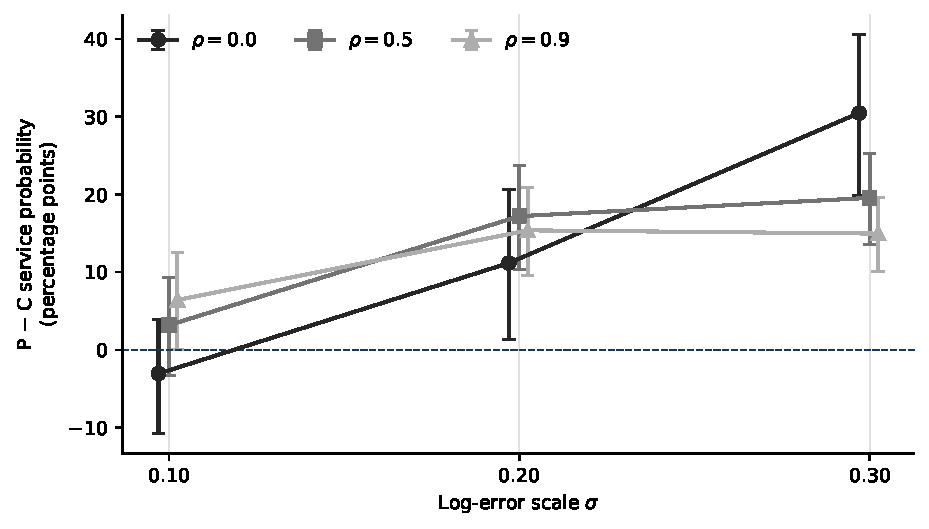
\includegraphics[width=0.93\textwidth]{Fig1.pdf}
 \caption{Paired difference in service probability between the original
 procedure (P) and conservative-speed planning (C) on the 46 common instances.
 Circles, squares and triangles mark $\rho=0$, $0.5$ and $0.9$, and the dashed
 line marks zero. Faint vertical lines mark $\sigma=0.10$, $0.20$ and $0.30$;
 markers are offset slightly around them only for legibility. Error bars are
 95\% bootstrap intervals over instances. Plans are fixed across this
 disturbance sweep, and the intervals are not simultaneous across cells.}
 \label{fig:reliability}
\end{figure}

\subsection{Confirmatory study}\label{sec:confirmatory}

The four hypotheses of the prespecified protocol were evaluated on 53 new instances (Table~\ref{tab:confirmatory}). Every decision uses the unrounded interval limits. The protocol's validation passed before any quantity was computed.

\begin{table}[htbp]
\centering
\footnotesize
\caption{Confirmatory results on 53 fresh instances. Differences are in percentage points of validated service-event probability; intervals are paired bootstrap intervals over instances. Conservative speed returned a plan on 50 of 53 instances, and H1 and H4 use those instances as the protocol defines.}
\label{tab:confirmatory}
\begin{tabular}{@{}>{\raggedright\arraybackslash}p{1.9cm}>{\raggedright\arraybackslash}p{4.2cm}>{\raggedright\arraybackslash}p{3.5cm}cc@{}}
\toprule
Hypothesis & Quantity & Estimate [interval] & Level & Decision\\
\midrule
H1 (primary) & Original procedure minus conservative speed, 50 instances & 15.7 [7.5, 23.6] & 97.5\% & confirmed\\
H2 (primary) & Capped minus original procedure, 53 instances & 11.7 [6.0, 17.9] & 97.5\% & confirmed\\
H3 & Admitted by capped / original procedure & 46 / 32 (capped only 14, original only 0) & exact $p=0.00012$ & confirmed\\
H4 & Advantage at $\sigma=0.30$ minus at $\sigma=0.10$ ($\rho=0$), 50 instances & 28.3 [19.6, 36.4] & 95\% & confirmed\\
\bottomrule
\end{tabular}
\end{table}

All four hypotheses were confirmed. The original procedure exceeded conservative speed by 15.7 points, capping exceeded the original procedure by 11.7 points, and capping admitted 46 instances against 32. Capping lost no instance that the original procedure admitted (14 gained, 0 lost). The advantage over conservative speed was 28.3 points larger at $\sigma=0.30$ than at $\sigma=0.10$ for independent disturbances. Of the plans admitted on the screening bank, 31 of 32 (original) and 45 of 46 (capped) retained the 0.95 lower bound on the fresh bank. Pooled over all instances, service probability was 79.4\% for the original procedure, 82.4\% for screened conservative speed and 91.0\% for the capped procedure, so the 95\% target is still not met on average. Screened conservative speed was not a prespecified comparison, and its pooled value is descriptive only. As in the development study, the shortfall comes from instances without an admitted plan. Plans admitted by screening averaged 97.4\% for the original procedure and 97.5\% for the capped procedure, while the fallback plans averaged 51.9\% (21 instances) and 48.7\% (7 instances).

H2 and H3 are not independent. When neither procedure admits a plan, both return the same fallback, and 11.6 of the 11.7 points of H2 come from the 14 instances that only the capped procedure admits. The two results are one finding measured twice.

\paragraph{Post hoc fallback.} The protocol fixes the fallback: without an admitted plan, both procedures return the uncontracted slack-aware plan. A variant that returns the conservative-speed plan instead, where that plan exists, would have raised pooled service on the same fresh bank from 79.4\% to 85.0\% for the original procedure (18 instances changed) and from 91.0\% to 93.0\% for the capped procedure (6 instances changed). The fallback rule uses no validation outcome, but this variant was chosen after the results were seen, so it is exploratory.

These instances come from the same generator and the same assumed disturbance model as the development study. The result establishes repeatability within that setting. It does not address real road networks, calibrated parameters or other instance families.

\subsection{Sensitivity to the objective weights}\label{sec:weights}

The original procedure was rerun on the 53 development instances with four weight vectors (Table~\ref{tab:weights}); neither confirmatory study varied the weights. Each rerun regenerates the candidate family, screens it on the same bank and validates the selected plan or fallback on the same fresh bank. Conservative-speed planning does not use the weights, so its archived outcome is reused. The rerun with the original weights differs from the archived run by $-$1.4 points pooled ([$-$5.1, 2.2]) and by one admitted instance (31 against 32). This is the run-to-run variation of a time-limited search.

\begin{table}[htbp]
\centering
\footnotesize
\setlength{\tabcolsep}{3pt}
\caption{Weight sensitivity on the 53 development instances. Weights are ordered distance cost, slack deficit, driver duration, fleet use. The advantage over conservative speed uses the 46 instances where conservative speed returned a plan. The last column is the paired difference in service probability from the rerun with the original weights, over all 53 instances (percentage points).}
\label{tab:weights}
\begin{tabular}{@{}>{\raggedright\arraybackslash}p{1.9cm}>{\raggedright\arraybackslash}p{4.4cm}>{\raggedright\arraybackslash}p{1.4cm}>{\raggedright\arraybackslash}p{1.3cm}>{\raggedright\arraybackslash}p{2.5cm}>{\raggedright\arraybackslash}p{2.5cm}@{}}
\toprule
Vector & Weights & Admitted & Pooled (\%) & Advantage over conservative [95\%] & Paired difference [95\%]\\
\midrule
Original (rerun) & (0.5693, 0.2643, 0.1055, 0.0609) & 31 & 77.5 & 16.2 [9.2, 22.8] & --\\
Slack first & (0.2643, 0.5693, 0.1055, 0.0609) & 30 & 77.4 & 16.0 [9.6, 22.1] & $-$0.1 [$-$3.9, 3.3]\\
Distance heavy & (0.8, 0.1, 0.05, 0.05) & 29 & 74.3 & 12.7 [5.3, 19.7] & $-$3.2 [$-$7.1, 0.2]\\
Equal & (0.25, 0.25, 0.25, 0.25) & 23 & 68.7 & 6.3 [$-$1.1, 13.7] & $-$8.8 [$-$14.3, $-$3.5]\\
\bottomrule
\end{tabular}
\end{table}

Swapping the two largest weights changed nothing beyond the run-to-run variation. The distance-heavy vector gave pooled service 3.2 points lower, with a paired interval that includes zero, and its advantage over conservative speed stayed clearly positive (12.7 [5.3, 19.7]). Equal weights changed the most. They admitted 23 instances against 31, lowered pooled service by 8.8 points (paired interval $-$8.8 [$-$14.3, $-$3.5]; $-$15.6 to $-$2.4 after adjusting the level for three comparisons), and left an advantage over conservative speed whose interval includes zero (6.3 [$-$1.1, 13.7]). Of the instances whose admission differed, 9 were admitted only under the original weights and 1 only under equal weights (exact $p=0.021$, unadjusted; the adjusted threshold for three comparisons is 0.017).

This analysis is exploratory. It uses the development instances and four vectors, chosen without searching for the point at which the advantage disappears, and each vector was run once; the original and equal vectors were rerun later, below. Equal weights give fleet size and driver duration 0.25 each, against 0.06 and 0.11 in the original vector; the run below separates the two.

To find what breaks under equal weights, two further vectors were fixed before a new run on the same instances: the original vector with the fleet-use weight raised to 0.25, and the original vector with the driver-duration weight raised to 0.25, the other weights scaled in proportion (\texttt{code/weight\_bracketing.py}). Equal weights change both at once. The original and equal vectors were rerun on the same machine, so the four rows of Table~\ref{tab:bracket} are comparable with each other; the run also stored every candidate, which the earlier run did not.

\begin{table}[htbp]
\centering
\scriptsize
\setlength{\tabcolsep}{4pt}
\caption{Weight bracketing on the 53 development instances (exploratory). Advantage over conservative speed on the instances where it has a plan, paired difference in service from the original vector rerun on the same machine (percentage points), and, averaged over instances, the share of candidates whose screening lower bound reached 0.95 and the mean vehicles per candidate.}
\label{tab:bracket}
\begin{tabular}{@{}l>{\raggedright\arraybackslash}p{2.9cm}rrllrr@{}}
\toprule
Vector & Weights & Adm. & Pooled & Advantage [95\%] & Diff.\ from original & Pass (\%) & Veh.\\
\midrule
Original (rerun here) & (0.5693, 0.2643, 0.1055, 0.0609) & 32 & 78.7 & 17.5 [10.8, 23.9] & -- & 17.3 & 7.88\\
Equal (rerun here) & (0.25, 0.25, 0.25, 0.25) & 24 & 70.2 & 8.1 [1.1, 15.1] & $-$8.5 [$-$13.0, $-$4.5] & 9.0 & 7.24\\
Fleet weight raised & (0.4546, 0.2111, 0.0843, 0.25) & 27 & 73.2 & 11.7 [4.7, 18.6] & $-$5.6 [$-$10.1, $-$1.4] & 13.5 & 7.58\\
Duration weight raised & (0.4773, 0.2216, 0.25, 0.0511) & 25 & 69.9 & 7.4 [$-$0.6, 15.4] & $-$8.9 [$-$14.1, $-$4.2] & 11.8 & 7.71\\
\bottomrule
\end{tabular}
\end{table}

Rerun on the same machine, the original vector admitted 32 instances and the equal vector 24, and the advantage over conservative speed fell from 17.5 [10.8, 23.9] to 8.1 [1.1, 15.1] points. The earlier run (Table~\ref{tab:weights}) gave \WtEqualPCMean{} points with an interval from \WtEqualPCLo{} to \WtEqualPCHi{}, so in both runs equal weights cut the advantage by more than half, but whether its interval reaches zero differs between runs. Raising the driver-duration weight to 0.25, with the other weights scaled down, lowered service about as much as equal weights did ($-$8.9 [$-$14.1, $-$4.2] against $-$8.5 [$-$13.0, $-$4.5] points from the original vector), and raising the fleet weight cost $-$5.6 [$-$10.1, $-$1.4] points. The run cannot separate the two effects: the duration-raised vector minus the fleet-raised one was $-$3.3 [$-$10.2, 3.4] points. The stored candidates suggest why the duration weight matters. Compared at the same instance and buffer, the duration-heavy candidates used only 0.18 fewer vehicles, against 0.29 for the fleet-heavy ones, yet their success on the screening bank fell more (2.5 against 1.1 points): they shortened driver duration by 85 minutes per plan on average and raised the slack deficit, so less waiting time was left to absorb delays. A heavier duration weight thus appears to remove slack that screening relies on. Of the 53 runs with the original vector, 39 ran on the first day while other analyses were also running on the machine, and the other runs of the bracketing ran later with the machine otherwise idle; because OR-Tools stops at a wall-clock limit, this may affect the comparison slightly.

\subsection{Solomon instances}\label{sec:solomon}

The unchanged pipeline was run on eight 100-customer Solomon instances with the time-dependent profile and disturbance model of the study overlaid (Section~\ref{sec:confdesign}). Within its five-second budget, OR-Tools returned a nominal plan for five of the eight instances (Table~\ref{tab:solomon}). PyVRP/HGS finds a feasible plan for the other three, R101, R102 and RC105, within 40 seconds, so these outcomes are search limits of the generator and not infeasibility of the mapped instances. The failure policy records them as missing plans, and every dependent configuration is recorded as not attempted.

\begin{table}[htbp]
\centering
\small
\caption{Solomon instances: validated service-event probability (\%). A dash marks a configuration with no plan. \emph{Plan} states whether OR-Tools returned a nominal plan; \emph{Admitted} states whether screening admitted a plan for the original procedure, which otherwise returns the slack-aware fallback.}
\label{tab:solomon}
\begin{tabular}{@{}lccccccc@{}}
\toprule
Instance & Plan & Nominal & Conservative & Slack-aware & Original & Capped & Admitted\\
\midrule
R101 & no & -- & -- & -- & -- & -- & no\\
R102 & no & -- & -- & -- & -- & -- & no\\
R103 & yes & 14.5 & -- & 45.1 & 45.1 & 45.1 & no\\
R112 & yes & 29.4 & 78.0 & 53.7 & 99.4 & 99.4 & yes\\
RC104 & yes & 22.8 & 82.0 & 68.9 & 97.7 & 97.7 & yes\\
RC105 & no & -- & -- & -- & -- & -- & no\\
RC106 & yes & 19.9 & 65.0 & 42.1 & 42.1 & 42.1 & no\\
RC108 & yes & 28.3 & 80.7 & 51.5 & 98.8 & 98.8 & yes\\
\bottomrule
\end{tabular}
\end{table}

On the five instances with a plan, screening admitted a plan for three (R112, RC104 and RC108). Their validated service probability was 97.7 to 99.4\%, against 78.0 to 82.0\% for conservative speed and 22.8 to 29.4\% for nominal distance. On the other two, the procedure returned the slack-aware fallback: R103 (45.1\%; conservative speed returned no plan there, although HGS finds a feasible plan for its matrix) and RC106 (42.1\%), where it fell 22.9 points below conservative speed (65.0\%). Capping changed no result on any instance.

The eight instances are all the R1 and RC1 files available in the source repository. They give no basis for an interval estimate, and no Solomon comparison was prespecified. The admitted plans reached 97.7 to 99.4\% and the fallback plans 42.1 to 45.1\%, a split similar to that on the synthetic instances. The generator, however, returned no plan on a substantial share of these harder instances.

\subsection{Second confirmatory study}\label{sec:confirmatory2}

In the exploratory run on the 53 development instances, the HGS capped procedure with conservative fallback exceeded HGS conservative-speed planning by 27.0 points, with pooled service of 94.2\%. Table~\ref{tab:confirmatory2} gives the prespecified results on the 53 new instances of the second study.

\begin{table}[htbp]
\centering
\footnotesize
\caption{Second confirmatory study on 53 new instances. Differences are in percentage points of validated service-event probability; intervals are paired bootstrap intervals over instances. G1 uses the 49 instances where HGS conservative-speed planning returned a plan.}
\label{tab:confirmatory2}
\begin{tabular}{@{}>{\raggedright\arraybackslash}p{1.9cm}>{\raggedright\arraybackslash}p{4.4cm}>{\raggedright\arraybackslash}p{3.3cm}cc@{}}
\toprule
Hypothesis & Quantity & Estimate [interval] & Level & Decision\\
\midrule
G1 (primary) & HGS capped with conservative fallback minus HGS conservative, 49 instances & 27.9 [23.0, 32.8] & 97.5\% & confirmed\\
G2 (primary) & OR-Tools capped, conservative minus slack-aware fallback, 53 instances & 0.4 [$-$0.7, 2.1] & 97.5\% & not confirmed\\
G3 & OR-Tools uncapped, conservative minus slack-aware fallback, 53 instances & 3.8 [1.6, 6.2] & 95\% & confirmed\\
G4 & HGS minus OR-Tools, both capped with conservative fallback, 53 instances & $-$0.2 [$-$4.0, 3.7] & 95\% & estimate only\\
\bottomrule
\end{tabular}
\end{table}

G1 was confirmed. With the HGS generator, screening with capped contraction exceeded conservative padding by 27.9 points, and pooled service probability reached 91.5\% against 58.4\% for HGS conservative speed. Capping was essential with this generator: at 100 and 200 customers the HGS capped family was admitted on 18 of 18 instances, and the uncapped family on 3.

G2 was not confirmed. The OR-Tools capped procedure admitted a plan on 45 of 53 instances and fell back on 8. On 4 of those no conservative-speed plan existed, so both rules returned the same plan. On the remaining 4 the conservative fallback changed service probability by +5.4, $-$3.1, $-$12.0 and +30.0 points. The post hoc gain seen for the capped procedure in the first study did not replicate. For the uncapped procedure, which falls back more often, the conservative fallback helped (G3, 3.8 points).

Under the capped procedure with conservative fallback, the two generators differed by $-$0.2 points (G4), with a 95\% interval from $-$4.0 to 3.7. No equivalence margin was prespecified, so this interval bounds the difference but does not establish equivalence. The HGS $\beta=0$ plan, which lacks the slack term, was a weak fallback: the uncapped HGS procedure pooled 51.0\% with it and 74.7\% with the conservative fallback (descriptive).

\subsection{Gehring--Homberger instances}\label{sec:gh}

As a harder external check, the HGS pipeline of the second study was run on the 20 Gehring--Homberger instances of classes R1 and RC1 with 200 customers \cite{gehring1999} (\texttt{code/gh\_benchmark.py}; exploratory). The mapping follows the Solomon check, except that the depot horizon of 634 time units is scaled to the 600-minute shift and the coordinates are scaled so that the benchmark's unit-speed travel corresponds to 40~km/h; capacity and fleet are kept. On R1\_2\_1 and R1\_2\_2, where all or most windows are only 10 time units wide, neither the OR-Tools anchor solves nor HGS at conservative speed found a plan, so the procedure could not run there. Screening admitted a plan on 17 of the other 18 instances (Table~\ref{tab:gh}). Where conservative speed had a plan, the HGS capped procedure exceeded it by 15.1 [11.0, 19.1] points (18 instances), and over all 20 instances it pooled 87.2\% against 73.6\% for conservative speed and 34.9\% for the nominal plan.

\begin{table}[htbp]
\centering
\footnotesize
\setlength{\tabcolsep}{4pt}
\caption{Gehring--Homberger instances with 200 customers (exploratory, HGS pipeline): instances, instances where the anchor solves found a plan, instances admitted by screening, and pooled validated service-event probability (\%) of the HGS nominal plan, HGS conservative speed and the HGS capped procedure with conservative fallback. A missing plan scores zero.}
\label{tab:gh}
\begin{tabular}{@{}lrrrrrr@{}}
\toprule
Class & Inst. & Anchors & Admitted & Nominal & Conservative & Capped\\
\midrule
R1 & 10 & 8 & 7 & 42.1 & 68.0 & 77.0\\
RC1 & 10 & 10 & 10 & 27.6 & 79.3 & 97.4\\
\bottomrule
\end{tabular}
\end{table}

\subsection{Robust optimization comparator}\label{sec:robust}

Table~\ref{tab:robust} compares the robust plans with the screened procedures on the 45 development instances with 20, 50 and 100 customers, and Fig.~\ref{fig:robust} shows the trade-off between service and distance; the appendix lists every setting. Every distance, including those of the OR-Tools and HGS plans, is given relative to the nominal plan found by the robust search with $\Gamma=0$; the OR-Tools nominal plans are 1.7\% longer on average.

\begin{table}[htbp]
\centering
\footnotesize
\caption{Robust comparator on the 45 development instances (exploratory): number of instances with a plan, mean validated service-event probability (\%) by size and pooled, mean distance relative to the nominal plan of the robust search ($\Gamma=0$) and mean vehicles, both over instances with a plan. A missing plan scores zero. Relief denotes the robust model with reachability relief.}
\label{tab:robust}
\begin{tabular}{@{}>{\raggedright\arraybackslash}p{4.6cm}rrrrrrr@{}}
\toprule
Configuration & Plans & $n=20$ & $n=50$ & $n=100$ & Pooled & Dist. (\%) & Veh.\\
\midrule
Conservative speed (OR-Tools) & 39 & 57.8 & 51.1 & 57.2 & 55.5 & 4.8 & 6.56\\
Capped procedure (OR-Tools) & 45 & 81.6 & 80.1 & 97.5 & 84.6 & 9.3 & 6.76\\
Capped procedure, conservative fallback (HGS) & 45 & 90.5 & 94.8 & 98.0 & 93.6 & 12.5 & 7.11\\
Robust, box, $\theta=0.4$ & 37 & 90.3 & 72.5 & 47.9 & 75.0 & 7.0 & 6.54\\
Robust, box, $\theta=0.6$ & 29 & 93.0 & 46.1 & 29.9 & 63.3 & 10.8 & 6.59\\
Relief, $\Gamma=3$, $\theta=0.4$ & 45 & 89.2 & 87.5 & 92.5 & 89.4 & 7.1 & 7.18\\
Relief, box, $\theta=0.4$ & 45 & 90.3 & 90.0 & 95.7 & 91.4 & 7.6 & 7.31\\
Relief, $\Gamma=3$, $\theta=0.6$ & 45 & 97.6 & 97.5 & 98.7 & 97.8 & 11.4 & 7.78\\
Relief, box, $\theta=0.6$ & 45 & 97.8 & 98.4 & 99.4 & 98.4 & 12.4 & 8.04\\
Screened robust & 45 & 97.0 & 82.8 & 75.1 & 87.4 & 7.9 & 7.20\\
Screened robust with relief & 45 & 97.2 & 97.4 & 97.2 & 97.2 & 10.4 & 7.64\\
\bottomrule
\end{tabular}
\end{table}

The standard robust model fails on the larger instances. Under box uncertainty it has no robust plan on 8 of the 45 instances with $\theta=0.4$ and on 16 with $\theta=0.6$. These are exactly the instances on which some customer cannot be served on time even by a direct trip at its upper travel time, so no fleet size helps. Every smaller budget $\Gamma$ failed on exactly the same instances. This is the reachability obstruction that capped contraction addresses (Section~\ref{sec:capping}). The mildest box setting, $\theta=0.2$, the robust counterpart of conservative speed, still had no plan on 4 instances and pooled 60.4\%.

Reachability relief removes the obstruction. Every relieved setting has a plan on all 45 instances, and under box uncertainty with $\theta=0.4$ relief raised pooled service by 16.4 points (Table~\ref{tab:robust-contrasts}). On the 37 instances where the standard model had a plan, the two models returned the same routes, so the whole gain comes from the instances without a standard robust plan. The relieved robust plans then compete with the screened procedures. With $\Gamma=3$ and $\theta=0.4$ they exceeded the OR-Tools capped procedure by 4.8 points on average, with an interval from $-$1.4 to 11.6, and used 0.42 more vehicles per instance. Against the HGS capped procedure the protection level decides the comparison. With $\Gamma=3$, the $\theta=0.4$ setting was 4.2 points less reliable (interval $-$7.2 to $-$0.7), with 4.6\% less distance and 0.07 more vehicles, while the $\theta=0.6$ setting was 4.2 points more reliable (interval 1.3 to 7.7) and used 0.67 more vehicles.

\begin{table}[htbp]
\centering
\footnotesize
\caption{Paired contrasts on the 45 development instances (exploratory). Service differences are in percentage points over all instances; distance differences are percentage changes and vehicle differences are means, both over instances where both configurations have a plan. Intervals are 95\% paired bootstrap intervals over instances.}
\label{tab:robust-contrasts}
\begin{tabular}{@{}>{\raggedright\arraybackslash}p{5.6cm}lll@{}}
\toprule
Contrast & Service [95\%] & Distance (\%) [95\%] & Vehicles\\
\midrule
Relief minus standard, box, $\theta=0.4$ & 16.4 [6.3, 27.1] & 0.0 [0.0, 0.0] & 0.00\\
Relief, $\Gamma=3$, $\theta=0.4$, minus OR-Tools capped procedure & 4.8 [$-$1.4, 11.6] & $-$1.7 [$-$3.4, 0.1] & 0.42\\
Relief, $\Gamma=3$, $\theta=0.4$, minus HGS capped procedure & $-$4.2 [$-$7.2, $-$0.7] & $-$4.6 [$-$6.0, $-$3.1] & 0.07\\
Relief, $\Gamma=3$, $\theta=0.6$, minus HGS capped procedure & 4.2 [1.3, 7.7] & $-$0.8 [$-$2.2, 0.8] & 0.67\\
Screened robust with relief minus HGS capped procedure & 3.6 [0.6, 7.1] & $-$1.6 [$-$3.0, $-$0.2] & 0.53\\
Screened robust with relief minus relief, box, $\theta=0.6$ & $-$1.1 [$-$1.5, $-$0.8] & $-$1.8 [$-$2.3, $-$1.2] & $-$0.40\\
\bottomrule
\end{tabular}
\end{table}

The screening layer can also wrap the robust generator. Screened robust with relief was admitted by screening on 44 of 45 instances and pooled 97.2\%, 3.6 points above the HGS capped procedure (interval 0.6 to 7.1), with 0.53 more vehicles. Against the most protective relieved setting it gave up 1.1 points and saved 1.8\% of distance, because it selects the shortest plan that passes the screen. Without relief, screening admitted a robust plan on 29 instances and pooled 87.4\%.

This comparison is exploratory. It uses the development instances, the grid was fixed before the runs, and the configurations in Table~\ref{tab:robust} are highlighted from that grid, which is reported in full. The robust plans minimize distance alone, without the slack, duration and fleet terms of the screened procedures, so differences in vehicles are part of the comparison.

\begin{figure}[ht]
 \centering
 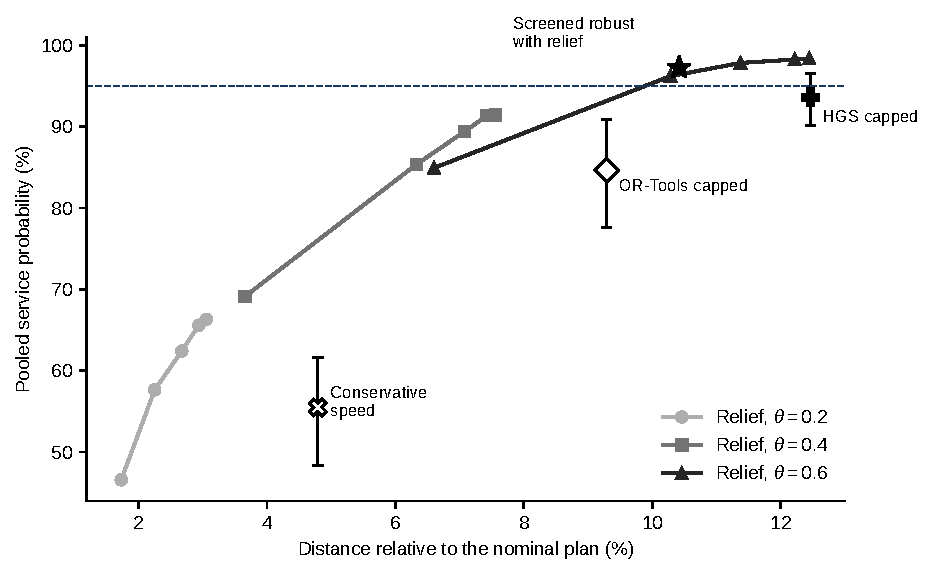
\includegraphics[width=0.93\textwidth]{Fig2.pdf}
 \caption{Pooled validated service-event probability against mean distance relative to the nominal plan of the robust search, on the 45 development instances. Lines join the relieved robust settings for each $\theta$, from $\Gamma=1$ to box uncertainty. The screened procedures (OR-Tools, HGS), screened robust with relief and conservative speed are shown separately. The dashed line marks the 95\% target}
 \label{fig:robust}
\end{figure}

With 200 customers, the relieved model was run on the 8 development instances with a reduced grid: $\Gamma=3$ and box uncertainty, each at $\theta=0.4$ and $0.6$, with 2000 iterations (median 114~s per solve). At $\theta=0.4$ the two budgets pooled 93.2\% and 96.1\%. At $\theta=0.6$ they pooled 86.8\% and 87.2\%, because the search found no plan for one instance under either budget; at this size relief does not guarantee a plan, and the search alone does not show whether that model is infeasible. Screened robust over the four settings admitted a plan on 7 instances and pooled 97.8\% with 20.6 vehicles on average, against 97.2\% with 17.0 vehicles for the HGS capped procedure and 97.6\% with 19.1 for the OR-Tools capped procedure on the same instances. With eight instances these figures are descriptive only.

\subsection{Robust comparison on the confirmatory instances}\label{sec:parta}

Part A of the third protocol \cite{ali2026freeze3} tested the development findings on the 90 confirmatory instances with up to 100 customers. Table~\ref{tab:parta} gives the prespecified results.

\begin{table}[htbp]
\centering
\footnotesize
\setlength{\tabcolsep}{4pt}
\caption{Third protocol, part A: prespecified results on the confirmatory instances with up to 100 customers. R1 and R4 use all instances of both studies; R2 and R3 use the second study, where HGS plans exist.}
\label{tab:parta}
\begin{tabular}{@{}l>{\raggedright\arraybackslash}p{5.6cm}lll@{}}
\toprule
Hypothesis & Quantity & Mean [interval] & Level & Decision\\
\midrule
R1 (primary) & Screened robust with relief minus OR-Tools capped, service & 6.7 [3.0, 11.1] & 97.5\% & confirmed\\
R2 (primary) & Screened robust with relief minus HGS capped, service & 6.7 [2.2, 12.2] & 97.5\% & confirmed\\
R3 & Screened robust with relief minus HGS capped, vehicles & 0.42 [0.20, 0.67] & 95\% & confirmed\\
R4 & Screened robust with relief vs. relief box $\theta=0.6$, distance (\%) & $-$1.3 [$-$1.7, $-$0.9] & 95\% & confirmed\\
\bottomrule
\end{tabular}
\end{table}

All four hypotheses met their decision criteria. Screened robust with relief pooled 97.2\%, against 90.5\% for the OR-Tools capped procedure and 98.4\% for the most protective relieved setting; on the second study the HGS capped procedure pooled 90.6\%. Screening admitted a robust plan on 86 of 90 instances.

Restricting the robust plans to the comparator's fleet removed much of their advantage. For each instance, the relieved settings were limited to plans that use no more vehicles than the comparator's plan, and the screened-robust rule was applied within that limit (\texttt{code/robust\_fleet\_matched.py}; exploratory, not part of the protocol). The limit also removes the most protective settings on many instances, so the comparison is not a pure fleet effect. On the development instances the restricted plans differed from the HGS capped procedure by $-$1.9 [$-$5.1, 1.5] points in service, with 3.8\% less distance, and from the OR-Tools capped procedure by 2.5 [$-$2.7, 8.1] points on the 43 instances with such a plan; screening admitted a restricted plan on 20 and 15 instances. On the confirmatory instances of part A the differences were 3.2 [$-$1.1, 8.1] points against the HGS capped procedure (45 instances, 28 admitted) and $-$0.7 [$-$3.9, 2.7] against the OR-Tools capped procedure (87 instances, 41 admitted). Every interval includes zero, so with no larger fleet than the comparator the robust plans were not measurably more reliable.

\subsection{Fallback rule}\label{sec:fallback}

When screening admits no candidate, each procedure returns a fixed fallback: the uncontracted slack-aware plan for the OR-Tools procedures and the conservative-speed plan for the HGS procedure. These fallbacks are the main reason the procedures pool below the 95\% target. After the development study and both confirmatory studies, a third fallback rule was examined: return the candidate of the procedure's own family with the highest screening success (ties by the normalized score, then the smaller buffer). The rule uses only the screening evidence already computed, so the validation bank still judges the returned plan independently, and it changes nothing on instances where a plan was admitted. Table~\ref{tab:fallback} compares the rules on the stored records (\texttt{code/fallback\_policy.py}).

\begin{table}[htbp]
\centering
\footnotesize
\setlength{\tabcolsep}{4pt}
\caption{Fallback rules on the stored records (exploratory, post hoc): instances where screening admitted nothing, pooled validated service-event probability (\%) over all instances under the stored fallback, the conservative-speed plan and the best-screened candidate, and the paired difference best-screened minus stored with a 95\% bootstrap interval (percentage points).}
\label{tab:fallback}
\begin{tabular}{@{}ll>{\raggedleft\arraybackslash}p{1.2cm}rrrl@{}}
\toprule
Study & Procedure & Fallback inst. & Stored & Cons. & Best & Best minus stored\\
\midrule
Development & Original (OR-Tools) & 21 & 78.9 & 82.7 & 91.6 & 12.7 [7.9, 17.9]\\
Development & Capped (OR-Tools) & 11 & 86.6 & 88.7 & 95.1 & 8.5 [4.0, 13.7]\\
Development & HGS capped & 5 & 94.2 & 94.2 & 97.2 & 3.0 [0.6, 5.7]\\
Confirmatory 1 & Original (OR-Tools) & 21 & 79.4 & 85.0 & 93.2 & 13.9 [9.0, 19.1]\\
Confirmatory 1 & Capped (OR-Tools) & 7 & 91.0 & 93.0 & 96.6 & 5.6 [1.9, 9.9]\\
Confirmatory 2 & Original (OR-Tools) & 25 & 77.1 & 80.9 & 92.7 & 15.6 [10.7, 20.8]\\
Confirmatory 2 & Capped (OR-Tools) & 8 & 91.4 & 91.7 & 96.2 & 4.9 [1.8, 8.5]\\
Confirmatory 2 & HGS capped & 8 & 91.6 & 91.6 & 96.1 & 4.6 [1.6, 8.1]\\
\bottomrule
\end{tabular}
\end{table}

The best-screened rule raised pooled service for every study and procedure, by 3.0 to 15.6 points, and every interval lies above zero. With it the capped procedures pooled 95.1 to 97.2\%. On the fallback instances themselves its plans averaged 83.0 to 95.0\%, against 45.2 to 62.9\% for the stored fallbacks. The conservative-speed fallback helped less. Because the rule was chosen after these results were known, part B of the third protocol tested it on new instances.

Part B ran the frozen OR-Tools and HGS pipelines on 53 new instances (development seeds plus 120000) under the third protocol \cite{ali2026freeze3}. Table~\ref{tab:partb} gives the prespecified results.

\begin{table}[htbp]
\centering
\footnotesize
\setlength{\tabcolsep}{4pt}
\caption{Third protocol, part B: prespecified results on the new instances. Differences and pooled service are in percentage points and percent; intervals are paired bootstrap intervals over instances.}
\label{tab:partb}
\begin{tabular}{@{}l>{\raggedright\arraybackslash}p{5.6cm}lll@{}}
\toprule
Hypothesis & Quantity & Mean [interval] & Level & Decision\\
\midrule
F1 (primary) & OR-Tools capped, best-screened minus slack-aware fallback & 7.3 [2.3, 13.2] & 97.5\% & confirmed\\
F2 (primary) & HGS capped, best-screened minus conservative fallback & 4.2 [1.2, 8.0] & 97.5\% & confirmed\\
F3 (estimate) & Pooled service, OR-Tools capped with best-screened fallback & 94.4 [90.1, 97.1] & 95\% & --\\
F4 (estimate) & Pooled service, HGS capped with best-screened fallback & 94.9 [91.0, 97.1] & 95\% & --\\
\bottomrule
\end{tabular}
\end{table}

Screening admitted nothing on 9 instances for the OR-Tools capped procedure and on 8 for the HGS capped procedure. With their stored fallbacks the two procedures pooled 87.1\% and 90.7\%; with the best-screened fallback they pooled 94.4\% and 94.9\%. Both primary hypotheses met their decision criteria. The pooled estimates stay just below 95\%. One instance cost more than the whole shortfall: there the OR-Tools anchor solves that fix the scaling ranges found no plan, so neither procedure could run and the instance scores zero, as the failure policy requires. On the other 52 instances the two procedures with the best-screened fallback pooled 96.3\% and 96.7\%; these figures are descriptive and were not prespecified. Both halves ran on a two-core Linux machine (Section~\ref{sec:conf3design}). The first stage was interrupted once by a restart of that machine; the frozen drivers resume from the records already written, so the completed instances were kept and the rest were run afterwards.

\subsection{Further checks}\label{sec:checks-summary}

Appendix~\ref{sec:checks} reports three further exploratory checks. Repeating the selection with a Bonferroni bound over the 13 buffer levels removed all 11 admitted plans that later missed the validation bound, while one newly selected plan fell below it, at the cost of 12 admissions and at most 1.8 points of pooled service. Screening a candidate took 3 to 24~ms, against seconds for generating it. Under four other delay models, the advantage of the capped procedures over conservative speed held for fixed plans. When the stored candidates were screened again under each model, the procedure with its stored fallback fell up to 19.0 points below the fixed plans, while with the best-screened fallback of Section~\ref{sec:fallback} it pooled between 93.2 and 96.7\% (Appendix~\ref{sec:misspec}).


Appendix~\ref{sec:additional} reports the results of the first two confirmatory studies by
size (Tables~\ref{tab:conf-size} and~\ref{tab:study2-size}, descriptive only), every robust setting
(Table~\ref{tab:robust-grid}), customer outcomes on the matched
subset (Table~\ref{tab:customers}), absolute planned resources
(Table~\ref{tab:fullcost}), service-threshold sensitivity
(Table~\ref{tab:kappa}), the instance-level failure audit
(Table~\ref{tab:failure}), and the equal-budget deterministic benchmark against
PyVRP/HGS (Table~\ref{tab:hgs}).

\section{Reproducibility and implementation checks}\label{sec:reproducibility}

The study archive \cite{ali2026archive} contains the candidate generators, the
scenario-bank code, the test suite, the experiment drivers, the raw JSON records
and the scripts that produce the results tables and the figures. The tests cover
FIFO behaviour, lognormal moments, common random numbers that do not depend on
evaluation order, Wilson calculations, visit and capacity feasibility, the rule
that contracted candidates are scored against the original windows, and the
robust feasibility checks, which are compared with brute-force enumeration of
deviation sets. Each run
records the Python, NumPy and OR-Tools versions, the operating system, the solver
budget, the seeds and the scenario counts.

The clock convention matters for reproduction. Relative time zero is 06:00, and
the evaluator adds 360 minutes before looking up the full-day speed profile;
leaving out that offset would evaluate a 00:00--10:00 shift instead. The
vectorized evaluator is checked against the original scalar implementation,
including period boundaries, customer lateness and shared arc disturbances.

Seeds are fixed. Admission uses seed $100000$ plus the instance seed, all
validation uses 5000 fresh scenarios from seed $400000$ plus the instance seed,
and the 1000-scenario disturbance sweep uses seed $500000$ plus the instance
seed. The capped, screened-conservative and clock-aware configurations were specified
before they were run on the development instances, but earlier aggregate results
motivated them, so they are exploratory and are neither preregistered nor an
external replication; the fresh scenario draws do not
remove the reuse of the instance set. Plans in the sweep are not re-screened when
$\sigma$ or $\rho$ changes.

The first confirmatory protocol (Section~\ref{sec:confdesign}) was publicly
timestamped, with a hash manifest of the code that runs and analyses it, before
its instances were solved; its results are in Section~\ref{sec:confirmatory}. One
pipeline smoke test, on an instance outside the confirmatory set, was run while
the protocol was being prepared, and the protocol discloses it as pilot data. The
confirmatory study used only frozen scripts. The weight-sensitivity analysis was
run after the freeze with a script outside the frozen file list. Its first run
stopped on a coding error that affected only that script, and the corrected
script produced the reported results. The second confirmatory study
(Section~\ref{sec:conf2design}) has its own frozen protocol and manifest. Its
OR-Tools half uses the frozen scripts of the first study, and its HGS half is
deterministic given the scaling ranges. The script that writes its tables and
text stops unless its verdicts and counts equal the saved output of the frozen
analysis and its estimates agree with that output to its two-decimal rounding.
The one-decimal figures in the paper are rounded from the exact estimates, and
those of the first study are produced in the same way. The development robust comparison (Section~\ref{sec:robust-design}) was run after
both studies with code outside the frozen file lists. Its search stops after a
fixed number of iterations with a fixed seed, so its plans are deterministic, and
the script that writes its tables and figure checks that every record is present
and complete. The third protocol (Section~\ref{sec:conf3design}) and its manifest
were committed publicly and archived \cite{ali2026freeze3} before any of its
runs; part B started one minute after the release. Its OR-Tools half was
interrupted once by a restart of the machine; the frozen drivers resume from the
records already written, so completed instances were kept and the remaining ones
were run afterwards. Both analysis programs ran once in confirmatory mode, after
all records were complete.

All results tables and both figures are regenerated from the retained records. Internal
planning buffers are always evaluated against the offered windows, candidate
selection and final assessment use independent banks, and solver-quality
comparisons between OR-Tools and HGS use equal wall-clock budgets on identical
deterministic instances. These rules stop diagnostics and within-run selection
from using their own validation outcomes. The robust search is compared with HGS
at fixed iteration counts. The family-wise, timing and misspecification checks
(Appendix~\ref{sec:checks}), the post hoc fallback comparison, the fleet-matched
robust contrast, the weight bracketing and the Gehring--Homberger check also use
code outside the frozen lists. The family-wise script first repeats every stored selection with
the original bound and stops unless all of them match, and the evaluator for the
alternative delay models reproduces the stored validation results exactly when
given the paper's model and validation seeds. A test checks this on OR-Tools,
HGS and robust plans of every instance size.

Reproducibility shows that the reported numbers follow from the archived code and
records. It does not show that the synthetic instances or the assumed disturbance
model represent a real operation; that needs the evidence listed in
Section~\ref{sec:limitations}.

\section{Limitations}\label{sec:limitations}

The study has eight main limitations.

First, the generators plan on nominal or iteratively frozen matrices, so the
procedure can miss better stochastic plans. The OR-Tools generator is also below
the state of the art: under an equal five-second budget, its routes are about
11\% longer than those of PyVRP/HGS at 200 customers (Table~\ref{tab:hgs}).
Absolute distance premiums therefore include solver quality, and some uncertified
screening failures may be search limits. The second confirmatory study shows that
the reliability result also holds with an HGS generator. That generator omits
the slack-deficit term, so the two generators do not solve identical objectives.
The clock-aware approximation is not an exact time-dependent optimizer. Generator
and objective choices also differ between screened families, so the experiments
are not a full factorial decomposition of every design decision.

Second, the robust comparison covers one budgeted-uncertainty model with one
search configuration. Its prespecified test used the confirmatory instances with
up to 100 customers, whose comparator results had already been published, and
the runs with 200 customers are exploratory. The robust plans minimize distance
alone, so differences in vehicles mix method and objective; with no larger fleet
than the comparator the robust plans were not measurably more reliable, but that
restriction was examined after the fact. The distributionally robust and
riskiness-index methods \cite{jaillet2016,zhang2019} are not compared.

Third, the disturbance parameters are assumed and have not been calibrated to
fleet GPS residuals. The results hold for those values and are not operational
forecasts. Under four other delay models (Appendix~\ref{sec:misspec}), the fixed
plans of the capped procedures lost up to \MisCappedDrop{} points of service,
and the advantage over padding remained. Screening the stored candidates again
under each model left pooled service between \ResLoOrt{} and \ResHiHgs\% with the
best-screened fallback, but the candidate families were not regenerated, and
neither that check nor the exploratory $\sigma$--$\rho$ grid replaces local
calibration.

Fourth, the geometry is synthetic. The Solomon check covers only \SolomonN{}
instances with 100 customers, and the generator found plans for \SolomonPlans{}
of them. The Gehring--Homberger check adds 20 instances with 200 customers but
uses one benchmark family, the HGS pipeline and an assumed mapping of time and
distance; it does not replace a real road network. The confirmatory instances
share the generator and disturbance model of the development study, so they test
repeatability within that setting.

Fifth, the weights come from one preference vector. Under equal weights the
advantage over conservative speed fell by more than half, and in one of two runs
its interval reached zero (Section~\ref{sec:weights}). Raising the
driver-duration weight alone had a similar effect. Only six vectors were tried,
and no confirmatory study varied the weights.

Sixth, Wilson screening accounts for binomial sampling error for a fixed
candidate. Its nominal coverage is not a simultaneous guarantee across an
adaptively searched grid, which is why held-out assessment is needed. With a
Bonferroni bound over the 13 buffer levels (Appendix~\ref{sec:familywise}),
admitted plans whose validation bound fell below 0.95 went from \FwMissOrig{} of
\FwAdmittedOrig{} to \FwMissFw{} of \FwAdmittedTotal{}, and at most
\FwLostMax{} admitted instances were lost per study and procedure. Screening also
does not prove feasibility if the disturbance distribution is misspecified.

Seventh, the evidence excludes breakdown recovery, heterogeneous fleets, insertion
of new orders, rolling-horizon replanning and departure-time recourse. Every
vehicle leaves at its planned time in every scenario, which makes the evaluation
stricter than an operator who adjusts departures would face.

Eighth, the fallback decides much of the procedure-level result. The
slack-aware plan prespecified in the first two studies can be worse than
conservative speed when screening admits nothing (Section~\ref{sec:solomon}),
and the conservative-speed fallback did not measurably improve the capped
procedure. The best-screened fallback, tested prospectively in the third
protocol, did improve both capped procedures, but pooled service stayed just
below 95\%, and the plans it returns have not passed the screen.

\section{Conclusion}

The development study separates three mechanisms. Uniformly conservative travel
times protect against predictable congestion by construction, but they pad every
trip, including off-peak ones. On matched instances the complete screened
procedure exceeded them by \ProcConsRange{} percentage points on average,
although the interval at 200 customers includes zero. For independent
disturbances its advantage grew with noise, from $\SweepLowIndep$ to
\SweepHighIndep{} points. The slack-aware objective without screening fell below
conservative speed, so the advantage comes from the complete procedure, in
which the contracted candidate family and statistical selection act together.
Screening also improves conservative speed: applied to conservative-speed
candidates, it performed about as well as the original procedure, and the capped
procedure had the highest service probability of the three
(Table~\ref{tab:screen}; exploratory). The fixed 20\% pad is therefore the weaker
of the two padding comparators.

In the first confirmatory study, on \ConfInstances{} new instances with
hypotheses fixed in a timestamped protocol before any of them was solved, all
four prespecified hypotheses met their protocol-defined decision criteria with the
original weight vector. H2 and H3 both measure the effect of capping, so
together they count as one finding. The screened procedure
exceeded conservative speed by \ConfHOneMean{} points (97.5\% interval
\ConfHOneLo{} to \ConfHOneHi{}). Capping added \ConfHTwoMean{} points
(\ConfHTwoLo{} to \ConfHTwoHi{}) and admitted \ConfHThreeK{} instances against
\ConfHThreeP{}, losing none. The advantage over conservative speed grew with
independent noise. These instances share the generator and the assumed
disturbance model of the development study, so the result shows repeatability
within that setting.

The advantage depends on the objective weights. Swapping the two largest weights
changed nothing beyond run-to-run variation, and a distance-heavy vector kept a
clearly positive advantage. With equal weights, fewer instances were admitted
(\WtEqualAdmitted{} against \WtBaseAdmitted{}), and the advantage over
conservative speed fell to \WtEqualPCMean{} points, with an interval from
\WtEqualPCLo{} to \WtEqualPCHi{}; a rerun on another machine gave
\BrEqAdv{} points (\BrEqAdvLo{} to \BrEqAdvHi{}). Raising the driver-duration
weight alone to 0.25 lowered service about as much as equal weights did
(\BrDurDiff{} against \BrEqDiff{} points), and raising the fleet weight alone
cost \BrFleetDiff{} points; the run cannot separate the two. The duration-heavy
candidates kept less waiting time to absorb delays. No confirmatory study varied the weights.

On \SolomonN{} Solomon instances with the same overlay, OR-Tools found a plan for
\SolomonPlans{}, and PyVRP/HGS found feasible plans for the other
\SolomonNoPlan{}. Screening admitted \SolomonAdmitted{} of the \SolomonPlans{}.
The admitted plans reached service probabilities near 98\%, and the fallback
plans stayed below 46\%. This exploratory check covers few instances, and it
shows that the candidate generator limits what the pipeline can do on harder
benchmarks. With HGS as generator, on \GhAttempted{} Gehring--Homberger instances
with 200 customers where the procedure could run, screening admitted a plan on
\GhAdmitted{}, and the procedure exceeded conservative speed by \GhDiff{} points
(95\% interval \GhDiffLo{} to \GhDiffHi{}; exploratory).

The second confirmatory study replaced OR-Tools with hybrid genetic search. With
that generator, screening with capped contraction exceeded conservative-speed
planning by \CtwoGOneMean{} points (97.5\% interval \CtwoGOneLo{} to
\CtwoGOneHi{}), and pooled service reached \CtwoPooledHGSK\% against
\CtwoPooledHGSCons\% for conservative speed. The HGS and OR-Tools procedures
differed by \CtwoGFourMean{} points, with a 95\% interval from \CtwoGFourLo{} to
\CtwoGFourHi{}. No equivalence margin was set, so this interval bounds the
difference but does not show equivalence. The reliability gain therefore
persists when HGS replaces OR-Tools, which makes it unlikely to be only an
artefact of a weak generator, although two generators do not show that it
holds for every solver. Capping mattered more with HGS: at 100 and 200
customers, its uncapped family was admitted on \CtwoHGSPAdmittedLarge{} of
\CtwoLarge{} instances and its capped family on \CtwoHGSKAdmittedLarge{}.

The fallback was the weakest part of the procedure as first specified. When
screening admits nothing,
the original protocol returns the uncontracted slack-aware plan, which on RC106
was far worse than conservative speed (Section~\ref{sec:solomon}). In the first
confirmatory study, a conservative-speed fallback examined post hoc would have
raised pooled service to \PostHocP\% for the original procedure and \PostHocK\%
for the capped procedure. Tested prospectively in the second study, this rule did
not measurably improve the capped procedure (G2, \CtwoGTwoMean{} points, interval
\CtwoGTwoLo{} to \CtwoGTwoHi{}). That procedure fell back on only
\CtwoORTKFallbacks{} instances, the rule changed the plan on
\CtwoFallbacksChanged{} of them, and the effects went both ways. The rule did
improve the uncapped procedure, by \CtwoGThreeMean{} points (95\% interval
\CtwoGThreeLo{} to \CtwoGThreeHi{}). A better rule uses the screening evidence
already computed: when nothing is admitted, return the candidate with the highest
screening success. Found post hoc, it raised pooled service in every study and
procedure, and in part B of the third protocol it met both prespecified decision
criteria on 53 new instances. It improved the OR-Tools capped procedure by
\PbFOne{} points (97.5\% interval \PbFOneLo{} to \PbFOneHi{}) and the HGS capped
procedure by \PbFTwo{} points (\PbFTwoLo{} to \PbFTwoHi{}), to pooled service of
\PbFThree\% and \PbFFour\%. Those estimates stay just below the 95\% target.
Looking at the instances afterwards, one instance on which neither procedure
could run costs more than the whole shortfall.

Screening failures can be diagnosed. Of the \FailureCount{} development instances
without an admitted plan, \CertifiedFailures{} meet a certified reachability
obstruction at one or more tested contraction levels. A certificate proves that
one particular contracted model is infeasible; it does not show that reachability
alone made the procedure miss its target. Capping each customer's contraction at
its direct-reachability limit raised admission from \OriginalSelected{} to
\CappedSelected{} instances. Of the instances with 100 or 200 customers,
\CappedLargeSelected{} were admitted and \CappedLargeRetained{} kept the target
lower bound under fresh validation, with mean service probability
\CappedLargeRange\%. The gain costs \CappedDistanceCost\% more distance and
\CappedFleetCost{} more vehicles on average, rising to \CappedFleetLarge{} more
vehicles at 200 customers. The earlier fleet-matched experiment concerns the
uncontracted objective and does not isolate the mechanism of the capped variant.
At 20 customers capping changes nothing. Only two of the six failures there meet
a certificate; of the other four, a longer search budget finds a plan for two,
and two remain unresolved.

Averaged over all instances, neither the original nor the capped procedure reaches
the 95\% target,
so both the procedure averages and the compliance of selected plans must be
reported. In the
development study, plans admitted by screening averaged \OriginalSelectedMean\%
for the original procedure and \CappedSelectedMean\% for the capped procedure,
while the fallback plans used on the other instances averaged
\OriginalFallbackMean\% and \CappedFallbackMean\%. All \CappedFallbackCount{}
capped-procedure fallbacks occur at 20 or 50 customers, so closing the remaining
gap depends on admitting plans for small instances. In the first confirmatory
study the capped procedure reached \ConfPooledK\% pooled, against \ConfPooledP\%
for the original procedure.

The robust comparison changes how the procedure should be read. A budgeted-robust
optimizer without relief had no plan on \RobNoPlanBoxSix{} of \RobInstances{}
development instances at its most protective setting, every time because some
customer could not be protected even on a direct trip. With the reachability
relief, the robust analogue of capped contraction, every setting had a plan on
the instances with up to 100 customers. Passed through the same screen, the relieved robust plans were more reliable than
both screened procedures, and part A of the third protocol confirmed this on
\PaInstances{} confirmatory instances with up to 100 customers (45 for the HGS
comparison): screened robust with relief exceeded the
OR-Tools capped procedure by \PaROne{} points (97.5\% interval \PaROneLo{} to
\PaROneHi{}) and the HGS capped procedure by \PaRTwo{} points (\PaRTwoLo{} to
\PaRTwoHi{}), and pooled \PaScreenedP\%. It used \PaRThree{} more vehicles per
instance than the HGS procedure, and when the robust plans were restricted to the
comparator's fleet they were not measurably more reliable (exploratory). The
screened procedures are therefore not the most reliable planners on these
instances. They offer a different trade-off: screening returns the shortest
candidate that passes a stated reliability test, while the robust plans' extra
reliability was no longer measurable when they could use no more vehicles than
the comparator. Within the robust family, screening
returned plans \PaRFourAbs\% shorter than the most protective setting, for
\PaBoxMinusScr{} points less service. What carries over between planners is
therefore the screening layer and the reachability relief, not a particular
generator.

Further exploratory checks qualify these findings. A family-wise bound over the
buffer grid removed all \FwMissOrig{} admitted plans that missed the validation
bound, while one newly selected plan missed it, and changed pooled service by
between \FwPooledChangeMin{} and \FwPooledChangeMax{} points. Screening a
candidate took milliseconds, against seconds for generating it. Under three of
four other delay models, fixed plans lost service, most under a stronger morning
peak and under incidents; the advantage over conservative speed held under all
four. When the stored candidates were screened again under each model, the stored
fallback made the procedure worse than the fixed plans under the harsher models,
by up to \ResWorstDrop{} points, while the best-screened fallback kept pooled
service between \ResLoOrt{} and \ResHiHgs\%. The lead of screened robust plans
over the HGS capped procedure was no longer distinguishable from zero under
time-of-day noise or the stronger peak.

These results depend on assumed disturbance parameters and synthetic geometry.
The development findings and the further checks were exploratory. The three
protocols support the main findings about the screened procedures, the
best-screened fallback and the robust comparison, within the prespecified
synthetic setting. Evidence from real road networks, other benchmark families
and calibrated disturbance parameters is still needed.

\section*{Acknowledgements}
The author thanks the researchers who answered methodological questions by
e-mail during the project.
These discussions informed experimental design; all claims in the paper rest
on the reported model, code, and experiments.

\section*{Statements and Declarations}

\paragraph{Competing interests.} The author has no relevant financial or non-financial interests to disclose.

\paragraph{Funding.} No funding was received for conducting this study.

\paragraph{Data and code availability.} The reproducibility archive contains
source code, dependency versions, tests, seeds, raw JSON records, analysis
scripts, generated tables and figures, and the three confirmatory protocols. It
is archived on Zenodo \cite{ali2026archive}; the code is released under the MIT
License and the records under CC BY 4.0. The three protocol freezes, each
archived before any run of its study, are separate records
\cite{ali2026freeze,ali2026freeze2,ali2026freeze3}. The Solomon and
Gehring--Homberger instance files in the archive are third-party benchmark data
\cite{solomon1987,ml4vrp2024,gehring1999} and remain under their original
terms.

\paragraph{Use of generative AI.} Generative AI assistants were used for
code development, experiment implementation, code review, analysis checking, and
drafting and editing text. They were OpenAI's ChatGPT (Astra 6) and Anthropic's
Claude (Opus 5, Opus 5.5 and Sonnet 5), and they are not authors. Every experiment
was run from the archived code, every reported number regenerates from the
archived raw records, and the headline results were recomputed independently of
the analysis scripts. Rerunning the solver can return different routes, because
each solve stops at a wall-clock limit; Section~\ref{sec:weights} measures this
run-to-run variation. The author reviewed all code and text and takes full
responsibility for the content.

\paragraph{Ethics approval.} Not applicable: the study uses synthetic and public
benchmark data only.

\paragraph{Consent.} Not applicable.

\paragraph{Author contributions.} S.A. is the sole author and conceived the
study, implemented the software, ran the experiments, and wrote the
manuscript.

\clearpage
\appendix
\section{Origin of the weight vector}\label{sec:ahp-matrix}

The baseline weights were first computed from an Analytic Hierarchy Process
matrix. They are used in this paper as a fixed experimental vector, and this
appendix records their origin only. Criteria are ordered as distance cost, slack deficit, driver duration and fleet
use. Entry $a_{kl}$ is the judged importance of criterion $k$ relative to $l$
on Saaty's 1--9 scale:
\[
\mathbf{A}=\begin{pmatrix}
1 & 3 & 5 & 7\\
1/3 & 1 & 3 & 5\\
1/5 & 1/3 & 1 & 2\\
1/7 & 1/5 & 1/2 & 1
\end{pmatrix}.
\]
Its principal eigenvalue is $\lambda_{\max}=4.0685$, and the normalised
principal eigenvector is
\[
\mathbf{w}=(0.5693,\;0.2643,\;0.1055,\;0.0609).
\]
With Saaty's random index 0.90 for four criteria, the consistency index is
$(4.0685-4)/3=0.0228$ and the consistency ratio is $0.0254$. As stated in Section~\ref{sec:objective-scaling},
the third row and column were set when the third criterion was total distance
and were not re-elicited for driver duration.

\section{Additional outcomes and failure records}\label{sec:additional}
\begin{table}[htbp]
\centering
\footnotesize
\caption{First confirmatory study by size (descriptive). For each procedure, the number of instances admitted by screening, the number of those that retained the 0.95 lower bound on the fresh bank in parentheses, and the mean validated service-event probability (\%) over all instances including fallbacks.}
\label{tab:conf-size}
\begin{tabular}{@{}rrrrrrrr@{}}
\toprule
$n$ & Inst. & \multicolumn{2}{c}{Original} & \multicolumn{2}{c}{Screened conservative} & \multicolumn{2}{c}{Capped}\\
\midrule
20 & 20 & 17/20 (17) & 90.2 & 15/20 (15) & 87.8 & 17/20 (17) & 90.2\\
50 & 15 & 8/15 (8) & 74.6 & 8/15 (8) & 80.3 & 12/15 (12) & 87.4\\
100 & 10 & 4/10 (3) & 71.3 & 3/10 (3) & 80.0 & 10/10 (9) & 97.1\\
200 & 8 & 3/8 (3) & 71.5 & 2/8 (2) & 75.4 & 7/8 (7) & 92.4\\
\bottomrule
\end{tabular}
\end{table}

\begin{table}[htbp]
\centering
\footnotesize
\caption{Second confirmatory study by size (descriptive): instances admitted by the capped procedure, and mean validated service-event probability (\%) over all instances, including fallbacks.}
\label{tab:study2-size}
\begin{tabular}{@{}rrrrrrrr@{}}
\toprule
$n$ & Inst. & \multicolumn{3}{c}{OR-Tools capped} & \multicolumn{3}{c}{HGS} \\ & & Admitted & Slack fb. & Cons. fb. & Admitted & Conservative & Capped, cons. fb.\\
\midrule
20 & 20 & 13 & 83.8 & 83.3 & 14 & 56.8 & 85.8\\
50 & 15 & 14 & 93.7 & 95.7 & 13 & 61.9 & 92.4\\
100 & 10 & 10 & 97.9 & 97.9 & 10 & 64.1 & 97.4\\
200 & 8 & 8 & 97.5 & 97.5 & 8 & 48.9 & 97.1\\
\bottomrule
\end{tabular}
\end{table}

\begin{table}[htbp]
\centering
\scriptsize
\caption{Every robust setting on the 45 development instances: instances with a plan, mean validated service-event probability (\%) by size and pooled, mean distance relative to the nominal plan and mean vehicles over instances with a plan. A missing plan scores zero.}
\label{tab:robust-grid}
\begin{tabular}{@{}lllrrrrrrr@{}}
\toprule
Model & $\theta$ & $\Gamma$ & Plans & $n=20$ & $n=50$ & $n=100$ & Pooled & Dist. (\%) & Veh.\\
\midrule
Nominal & 0 & 0 & 45 & 20.7 & 17.7 & 26.4 & 21.0 & 0.0 & 5.98\\
Standard & 0.2 & 1 & 41 & 47.3 & 37.9 & 40.8 & 42.7 & 1.6 & 6.02\\
Standard & 0.2 & 2 & 41 & 58.6 & 47.4 & 48.9 & 52.7 & 2.2 & 6.17\\
Standard & 0.2 & 3 & 41 & 63.2 & 50.3 & 54.6 & 57.0 & 2.6 & 6.34\\
Standard & 0.2 & 5 & 41 & 65.2 & 53.8 & 57.8 & 59.8 & 2.9 & 6.37\\
Standard & 0.2 & box & 41 & 65.3 & 54.2 & 59.8 & 60.4 & 3.0 & 6.32\\
Standard & 0.4 & 1 & 37 & 70.8 & 54.5 & 35.4 & 57.5 & 3.4 & 6.00\\
Standard & 0.4 & 2 & 37 & 86.0 & 67.2 & 43.6 & 70.3 & 5.8 & 6.19\\
Standard & 0.4 & 3 & 37 & 89.2 & 70.7 & 46.2 & 73.5 & 6.6 & 6.46\\
Standard & 0.4 & 5 & 37 & 90.5 & 72.2 & 47.6 & 74.9 & 6.9 & 6.57\\
Standard & 0.4 & box & 37 & 90.3 & 72.5 & 47.9 & 75.0 & 7.0 & 6.54\\
Standard & 0.6 & 1 & 29 & 82.5 & 39.0 & 25.3 & 55.3 & 5.6 & 5.62\\
Standard & 0.6 & 2 & 29 & 91.6 & 44.8 & 29.2 & 62.2 & 9.1 & 6.31\\
Standard & 0.6 & 3 & 29 & 92.7 & 45.8 & 29.6 & 63.1 & 9.9 & 6.38\\
Standard & 0.6 & 5 & 29 & 92.8 & 46.1 & 29.9 & 63.2 & 10.7 & 6.52\\
Standard & 0.6 & box & 29 & 93.0 & 46.1 & 29.9 & 63.3 & 10.8 & 6.59\\
Relief & 0.2 & 1 & 45 & 47.3 & 43.0 & 50.5 & 46.6 & 1.7 & 6.22\\
Relief & 0.2 & 2 & 45 & 58.6 & 54.0 & 61.2 & 57.6 & 2.3 & 6.36\\
Relief & 0.2 & 3 & 45 & 63.2 & 57.6 & 68.0 & 62.4 & 2.7 & 6.53\\
Relief & 0.2 & 5 & 45 & 65.2 & 62.2 & 71.5 & 65.6 & 2.9 & 6.58\\
Relief & 0.2 & box & 45 & 65.3 & 62.4 & 74.1 & 66.3 & 3.1 & 6.51\\
Relief & 0.4 & 1 & 45 & 70.8 & 66.1 & 70.1 & 69.1 & 3.7 & 6.53\\
Relief & 0.4 & 2 & 45 & 86.0 & 83.3 & 87.2 & 85.4 & 6.3 & 6.89\\
Relief & 0.4 & 3 & 45 & 89.2 & 87.5 & 92.5 & 89.4 & 7.1 & 7.18\\
Relief & 0.4 & 5 & 45 & 90.5 & 90.2 & 94.7 & 91.4 & 7.4 & 7.24\\
Relief & 0.4 & box & 45 & 90.3 & 90.0 & 95.7 & 91.4 & 7.6 & 7.31\\
Relief & 0.6 & 1 & 45 & 86.9 & 82.2 & 84.9 & 84.9 & 6.6 & 6.87\\
Relief & 0.6 & 2 & 45 & 96.5 & 95.2 & 97.3 & 96.2 & 10.3 & 7.64\\
Relief & 0.6 & 3 & 45 & 97.6 & 97.5 & 98.7 & 97.8 & 11.4 & 7.78\\
Relief & 0.6 & 5 & 45 & 97.7 & 98.3 & 99.3 & 98.2 & 12.2 & 7.96\\
Relief & 0.6 & box & 45 & 97.8 & 98.4 & 99.4 & 98.4 & 12.4 & 8.04\\
\bottomrule
\end{tabular}
\end{table}

\begin{table}[H]
\centering
\small
\caption{Customer outcomes on the instances where conservative-speed planning returned a plan. The clock approximation also excludes the instances where it found no schedule, and the counts show this.}
\label{tab:customers}
\begin{tabular}{lrll}
\toprule
Configuration & $k$ & On time (\%) & Expected late\\
\midrule
Nominal & 46 & 83.6 [82.5, 84.6] & 10.00 [7.95, 12.20]\\
Conservative speed & 46 & 93.9 [93.4, 94.4] & 3.47 [2.84, 4.14]\\
Slack-aware & 46 & 90.9 [90.0, 91.7] & 5.46 [4.38, 6.65]\\
Fleet-matched & 46 & 83.0 [81.9, 84.0] & 10.47 [8.29, 12.87]\\
Original procedure & 46 & 96.6 [95.1, 97.9] & 2.20 [1.26, 3.31]\\
Screened conservative & 46 & 97.1 [96.3, 97.8] & 2.20 [1.47, 2.99]\\
Capped procedure & 46 & 97.7 [96.4, 98.9] & 0.91 [0.56, 1.32]\\
Clock approximation & 44 & 88.0 [87.2, 88.7] & 6.73 [5.39, 8.23]\\
\bottomrule
\end{tabular}
\end{table}


\begin{table}[H]
\centering
\scriptsize
\caption{Mean absolute planned resources on the same instances as Table~\ref{tab:customers}: distance in km, scheduled duration in minutes, and vehicles. These are not claims of optimality.}
\label{tab:fullcost}
\begin{tabular}{lrlll}
\toprule
Configuration & $k$ & Distance & Duration & Fleet\\
\midrule
Nominal & 46 & 1180.7 [989.9, 1381.0] & 2906.5 [2379.9, 3481.3] & 7.67 [6.46, 8.98]\\
Conservative speed & 46 & 1216.2 [1021.5, 1422.0] & 3352.5 [2738.5, 4011.0] & 8.30 [6.93, 9.76]\\
Slack-aware & 46 & 1196.3 [1003.0, 1404.0] & 2902.0 [2380.3, 3466.2] & 7.46 [6.22, 8.78]\\
Fleet-matched & 46 & 1174.2 [989.2, 1372.8] & 2833.6 [2330.6, 3382.6] & 7.46 [6.22, 8.76]\\
Original procedure & 46 & 1247.9 [1049.3, 1453.0] & 3171.2 [2620.9, 3777.3] & 8.17 [6.89, 9.57]\\
Screened conservative & 46 & 1252.8 [1056.4, 1461.2] & 3494.5 [2874.0, 4161.0] & 8.76 [7.35, 10.28]\\
Capped procedure & 46 & 1283.5 [1076.5, 1506.8] & 3317.3 [2709.4, 3964.1] & 8.52 [7.13, 10.04]\\
Clock approximation & 44 & 1137.2 [955.5, 1330.9] & 2868.3 [2335.0, 3456.8] & 7.64 [6.32, 9.11]\\
\bottomrule
\end{tabular}
\end{table}


\begin{table}[H]
\centering
\scriptsize
\caption{Sensitivity to the service threshold $\kappa$ on the 46 common instances, with the same plans and the same fresh validation bank in every column. At $n=20/50/100/200$, the number of customers allowed to be late is $2/5/10/20$ at $\kappa=.90$, $1/2/5/10$ at $.95$, $0/1/2/4$ at $.98$, and zero at 1.00.}
\label{tab:kappa}
\begin{tabular}{rlllll}
\toprule
$\kappa$ & N & C & S & P & SC\\
\midrule
0.90 & 38.8 [36.5, 41.2] & 80.6 [78.8, 82.4] & 68.8 [65.9, 71.7] & 89.2 [84.2, 93.7] & 91.2 [88.5, 93.8]\\
0.95 & 21.9 [20.3, 23.5] & 65.6 [63.1, 68.0] & 52.8 [49.9, 55.8] & 83.1 [76.3, 89.4] & 82.8 [77.9, 87.6]\\
0.98 & 11.2 [10.3, 12.2] & 48.2 [45.6, 50.8] & 36.4 [33.8, 39.0] & 75.9 [68.2, 83.3] & 73.2 [67.1, 79.3]\\
1.00 & 6.4 [5.4, 7.4] & 34.4 [31.8, 37.0] & 26.1 [23.8, 28.5] & 68.2 [59.6, 76.2] & 62.4 [53.8, 70.9]\\
\bottomrule
\end{tabular}
\end{table}


\subsection{Instance-level failure audit}\label{sec:failure-audit}

\begin{table}[H]
\centering
\scriptsize
\caption{Every instance on which the original procedure admitted no plan. Best $\beta$ and the lower confidence bound (LCB) refer to the best returned candidate; the no-plan $\beta$ is the first buffer at which the solver returned no plan; the proof $\beta$ is the first buffer with a reachability certificate. Unresolved marks at least one no-plan result without a certificate. A dash means none up to 60 minutes.}
\label{tab:failure}
\begin{tabular}{rrrrrrc}
\toprule
$n$ & Seed & Best $\beta$ & LCB (\%) & No-plan $\beta$ & Proof $\beta$ & Unresolved\\
\midrule
20 & 7200 & 45 & 90.7 & 50 & -- & Yes\\
20 & 7201 & 35 & 93.5 & 40 & -- & Yes\\
20 & 7210 & 35 & 90.8 & 45 & -- & Yes\\
20 & 7212 & 5 & 37.9 & 10 & -- & Yes\\
20 & 7216 & 55 & 90.7 & 60 & 60 & No\\
20 & 7218 & 10 & 65.9 & 15 & 50 & Yes\\
50 & 7501 & 25 & 87.5 & 30 & 35 & Yes\\
50 & 7503 & 10 & 64.1 & 15 & 15 & No\\
50 & 7504 & 35 & 91.3 & 40 & 40 & No\\
50 & 7506 & 0 & 44.7 & 5 & 5 & No\\
50 & 7508 & 35 & 85.9 & 40 & 40 & No\\
50 & 7511 & 35 & 88.5 & 40 & 50 & Yes\\
50 & 7513 & 40 & 93.6 & 45 & 60 & Yes\\
100 & 8003 & 20 & 85.3 & 25 & 25 & No\\
100 & 8004 & 15 & 81.5 & 20 & 20 & No\\
100 & 8007 & 5 & 73.6 & 15 & 15 & No\\
100 & 8008 & 25 & 91.7 & 35 & 35 & No\\
200 & 9004 & 10 & 71.2 & 15 & 15 & No\\
200 & 9005 & 20 & 88.9 & 25 & 25 & No\\
200 & 9006 & 25 & 94.9 & 40 & 40 & No\\
200 & 9007 & 20 & 86.4 & 25 & 25 & No\\
\bottomrule
\end{tabular}
\end{table}


\begin{table}[H]
\centering
\small
\caption{Retained equal-budget benchmark on the deterministic core: excess distance of OR-Tools routes over PyVRP/HGS routes (\%). Counts are valid pairs at the one-second and five-second budgets; one pair is missing at one second.}
\label{tab:hgs}
\begin{tabular}{rrll}
\toprule
$n$ & Valid pairs (1s/5s) & One second & Five seconds\\
\midrule
20 & 19/20 & 1.0 [0.3, 1.8] & 0.0 [0.0, 0.0]\\
50 & 15/15 & 4.8 [3.3, 6.2] & 3.0 [1.9, 4.2]\\
100 & 10/10 & 8.5 [5.9, 11.1] & 6.3 [4.7, 7.9]\\
200 & 8/8 & 32.9 [29.4, 36.2] & 11.1 [9.3, 13.5]\\
\bottomrule
\end{tabular}
\end{table}

\clearpage
\section{Further exploratory checks}\label{sec:checks}

The three checks in this appendix were added after the first two confirmatory studies and are exploratory. The first reuses the stored screening counts, the second times screening and one HGS solve on each development instance and counts the selected buffers, and the third evaluates the stored plans on new scenarios. The misspecification check also reruns the selection under each alternative model.

\subsection{Family-wise screening}\label{sec:familywise}

The admission bound holds for each candidate separately, while the procedure searches 13 buffer levels per instance. To check whether this matters, every stored candidate family was screened again with the Wilson bound at $\eta/13$, a Bonferroni adjustment that makes the 95\% bound hold simultaneously over the grid. Selection and fallback were otherwise unchanged, and any newly selected plan was validated on the original fresh bank (Table~\ref{tab:familywise}). Over the 8 combinations of study and procedure, the adjustment reduced the admitted instances from 318 to 306, at most 2 per combination, and selected a different plan on 79 of the instances it still admitted. Admitted plans whose validation lower bound fell below 0.95 went from 11 of 318 to 1 of 306. Pooled service changed by between $-$1.8 and 0.2 points. Admitted plans averaged 97.3 to 98.0\% on the fresh bank under the per-candidate bound, depending on study and procedure, and 97.7 to 98.3\% under the family-wise bound. The stricter bound thus removed all 11 admitted plans whose validation bound fell below 0.95, while one plan it newly selected fell below it, at the cost of a few admissions and up to 1.8 points of pooled service.

\begin{table}[htbp]
\centering
\footnotesize
\setlength{\tabcolsep}{4pt}
\caption{Family-wise screening (exploratory). Adm.: instances with an admitted plan. Kept: admitted plans whose validation lower bound was at least 0.95. Pooled: validated service-event probability (\%) of the procedure over all instances, fallbacks included. Columns marked FW use the Bonferroni bound over the 13 buffer levels.}
\label{tab:familywise}
\begin{tabular}{@{}l>{\raggedright\arraybackslash}p{3.1cm}rrrrrr@{}}
\toprule
Study & Procedure & Adm. & Kept & Pooled & Adm.\ FW & Kept FW & Pooled FW\\
\midrule
Development & Original (OR-Tools) & 32 & 30 & 78.9 & 30 & 30 & 77.1\\
Development & Capped (OR-Tools) & 42 & 40 & 86.6 & 40 & 40 & 85.0\\
Development & HGS capped, conservative fallback & 48 & 46 & 94.2 & 46 & 46 & 93.2\\
Confirmatory 1 & Original (OR-Tools) & 32 & 31 & 79.4 & 30 & 30 & 77.8\\
Confirmatory 1 & Capped (OR-Tools) & 46 & 45 & 91.0 & 45 & 45 & 90.7\\
Confirmatory 2 & Original (OR-Tools) & 28 & 28 & 77.1 & 27 & 27 & 76.2\\
Confirmatory 2 & Capped (OR-Tools) & 45 & 45 & 91.4 & 45 & 44 & 91.6\\
Confirmatory 2 & HGS capped, conservative fallback & 45 & 42 & 91.6 & 43 & 43 & 90.6\\
\bottomrule
\end{tabular}
\end{table}

\subsection{Computation time and buffer choice}\label{sec:time}

Screening is cheap relative to generation. On one x86-64 Linux machine, evaluating one candidate on the 1000-scenario screening bank took a median of 3~ms at 20 customers and 24~ms at 200. A candidate solve has a fixed five-second OR-Tools budget, and a median HGS solve took 2.2~s at 20 customers and 9.3~s at 200. The procedure's cost therefore lies in up to 13 candidate solves ($\beta=0$ to 60 minutes), each of which OR-Tools repeats at most twice if it returns no plan. Absolute times depend on the machine.

Among admitted selections, the buffer grid was rarely binding for OR-Tools. Over the three studies, 191 of the 225 OR-Tools selections used a buffer between 25 and 45 minutes, and 4 used the largest buffer of 60 minutes; the median selected buffer was 35 minutes. HGS selected larger buffers (median 50 minutes), and 11 of its 93 selections were at 60 minutes, so a wider grid could change some HGS selections. On instances where nothing was admitted, no buffer up to 60 minutes passed, and the grid cannot show whether a larger one would have.

\subsection{Misspecified delay models}\label{sec:misspec}

The plans were screened under one assumed disturbance model. To test how much the conclusions depend on it, the stored plans of the development study and the first two confirmatory studies were evaluated, without re-screening or re-optimization, on 5000 new scenarios per instance under four other models. The models were chosen before the run, but they were not registered. The heavy-tail model replaces the normal common and local log-errors by Student-$t$ errors with three degrees of freedom, scaled to the same variance. At equal variance these errors are more peaked near zero and have heavier tails, so the model changes the shape of the distribution more than its spread; the multipliers then have infinite mean, although every simulated value is finite. The incident model adds, on each arc traversal, an independent 3\% chance that the travel time doubles. The time-of-day model uses $\sigma=0.30$ and $\rho=0.8$ for departures in the morning peak (07:00--09:00) and $\sigma=0.15$ and $\rho=0.3$ at other times, in place of $\sigma=0.20$ and $\rho=0.5$ throughout. (The code also raises the noise in the evening peak, which begins after every time window has closed and so has no effect.) The stronger-peak model divides speed by 1.4 between 07:00 and 09:00, where the plans assumed 1.2. Tables~\ref{tab:misspec} and~\ref{tab:misspec-contrasts} pool the 159 OR-Tools instances, the 106 HGS instances and the 45 instances of the robust comparison.

\begin{table}[htbp]
\centering
\footnotesize
\setlength{\tabcolsep}{4pt}
\caption{Misspecified delay models (exploratory): pooled service-event probability (\%) of fixed plans on 5000 new scenarios per instance. OR-Tools columns use 159 instances, HGS columns 106 and screened robust with relief 45; because the instance sets differ, configurations are compared in Table~\ref{tab:misspec-contrasts}. Cons.: conservative speed. Original and Capped: the OR-Tools procedures. HGS capped: the HGS capped procedure with conservative fallback. A missing plan scores zero.}
\label{tab:misspec}
\begin{tabular}{@{}lrrrrrr@{}}
\toprule
Delay model & Cons. & Original & Capped & HGS cons. & HGS capped & Scr.\ robust\\
\midrule
Paper's model (new scenarios) & 57.8 & 78.5 & 89.7 & 59.6 & 92.9 & 97.2\\
Heavy tails & 64.0 & 79.8 & 89.9 & 65.8 & 93.6 & 97.3\\
Incidents & 49.6 & 71.7 & 84.6 & 51.1 & 87.5 & 92.2\\
Time-of-day noise & 56.4 & 77.6 & 88.4 & 58.3 & 91.3 & 93.5\\
Stronger morning peak & 36.8 & 67.1 & 82.9 & 38.4 & 86.0 & 90.8\\
\bottomrule
\end{tabular}
\end{table}

\begin{table}[htbp]
\centering
\footnotesize
\setlength{\tabcolsep}{4pt}
\caption{Misspecified delay models (exploratory): paired differences in service probability (percentage points) with 95\% bootstrap intervals over instances. Cons.: conservative speed.}
\label{tab:misspec-contrasts}
\begin{tabular}{@{}>{\raggedright\arraybackslash}p{2.5cm}>{\raggedright\arraybackslash}p{2.3cm}>{\raggedright\arraybackslash}p{2.3cm}>{\raggedright\arraybackslash}p{2.4cm}>{\raggedright\arraybackslash}p{2.4cm}@{}}
\toprule
Delay model & Original minus cons. & Capped minus cons. & HGS capped minus HGS cons. & Scr.\ robust minus HGS capped\\
\midrule
Paper's model (new scenarios) & 20.7 [16.7, 24.7] & 31.9 [28.3, 35.6] & 33.3 [29.0, 38.0] & 3.6 [0.7, 7.0]\\
Heavy tails & 15.8 [11.5, 20.0] & 25.8 [21.9, 29.8] & 27.8 [23.3, 32.7] & 3.1 [0.8, 5.7]\\
Incidents & 22.1 [18.1, 26.1] & 35.0 [31.5, 38.5] & 36.4 [32.3, 40.7] & 4.5 [1.2, 8.4]\\
Time-of-day noise & 21.2 [17.4, 25.0] & 32.0 [28.5, 35.5] & 32.9 [28.7, 37.5] & 1.7 [$-$1.0, 5.1]\\
Stronger morning peak & 30.3 [25.5, 35.1] & 46.1 [42.0, 50.1] & 47.7 [43.0, 52.3] & 3.6 [$-$1.0, 9.1]\\
\bottomrule
\end{tabular}
\end{table}

Heavy tails did not lower service. Conservative speed gained most, from 57.8 to 64.0\% for OR-Tools, and the capped procedures and screened robust changed by less than one point. The other three models lowered service for every configuration, most of all the stronger peak and then incidents. The stronger peak reduced the capped procedures by up to 6.9 points and conservative speed by up to 21.2 points: travel in the morning peak now takes 40\% longer than at nominal speed, which the 20\% pad no longer covers. The advantage over conservative speed held under every model, with lower interval limits of at least 11.5 points for the original procedure, 21.9 for the capped procedure and 23.3 for the HGS capped procedure. On its 45 instances, screened robust with relief stayed ahead of the HGS capped procedure under every model, but its lead fell from 3.6 to 1.7 points under time-of-day noise, and the intervals include zero under time-of-day noise and the stronger peak. These results concern fixed plans.

Re-screening asks what the procedure itself would do under each model. Every stored candidate of the capped families was screened again on 1000 scenarios drawn from that model (seed 100000 plus the instance seed), the selection rule was applied unchanged, and the selected plan was validated on the same 5000 scenarios of that model. The candidate families were not regenerated. Under the paper's model this reproduces every stored selection, which the script checks. Table~\ref{tab:rescreen} reports two fallbacks for instances where nothing is admitted: the procedure's stored fallback, and the candidate with the highest screening success (Section~\ref{sec:fallback}).

\begin{table}[htbp]
\centering
\footnotesize
\setlength{\tabcolsep}{4pt}
\caption{Re-screening under each delay model (exploratory): pooled service-event probability (\%) of the capped procedures over 159 OR-Tools and 106 HGS instances. Fixed: the stored plans. Re-screened: the stored candidates screened again under the model, with the stored fallback. Best: the same, with the best-screened fallback.}
\label{tab:rescreen}
\begin{tabular}{@{}lrrrrrr@{}}
\toprule
Delay model & \multicolumn{3}{c}{OR-Tools capped} & \multicolumn{3}{c}{HGS capped}\\
 & Fixed & Re-screened & Best & Fixed & Re-screened & Best\\
\midrule
Paper's model (new scenarios) & 89.7 & 89.7 & 96.0 & 92.9 & 92.9 & 96.7\\
Heavy tails & 89.9 & 91.3 & 96.0 & 93.6 & 93.8 & 96.5\\
Incidents & 84.6 & 69.4 & 93.2 & 87.5 & 68.5 & 93.7\\
Time-of-day noise & 88.4 & 86.8 & 95.4 & 91.3 & 88.5 & 96.1\\
Stronger morning peak & 82.9 & 72.8 & 93.5 & 86.0 & 72.4 & 94.8\\
\bottomrule
\end{tabular}
\end{table}

With the stored fallback, re-screening did worse than keeping the fixed plans under incidents and the stronger peak, by up to 19.0 points, and for HGS also under time-of-day noise. Fewer candidates passed under these models (OR-Tools 81 and 102 admissions against 133 under the paper's model), and the instances that failed received the weak stored fallback. With the best-screened fallback, re-screening exceeded the fixed plans under every model, and pooled service stayed between 93.2 and 96.0\% for OR-Tools and between 93.7 and 96.7\% for HGS.

\clearpage

\begingroup
\small

\bibliographystyle{sn-basic}
\bibliography{sn-bibliography}
\endgroup

\end{document}
